% SIAM Article Template
\documentclass[review,onefignum,onetabnum]{siamonline171218}

% Information that is shared between the article and the supplement
% (title and author information, macros, packages, etc.) goes into
% ex_shared.tex. If there is no supplement, this file can be included
% directly.

% SIAM Shared Information Template
% This is information that is shared between the main document and any
% supplement. If no supplement is required, then this information can
% be included directly in the main document.


% Packages and macros go here
\usepackage{lipsum}
\usepackage{amsfonts}
\usepackage{graphicx}
\usepackage{epstopdf}
\usepackage{algorithm}      % for floating algorithm environment
\usepackage{algpseudocode}  % for the algorithmicx syntax (\State, \While, etc.)
\usepackage{mathtools}
\usepackage{booktabs}
\usepackage{subcaption}
\usepackage[scr=rsfs]{mathalpha}
\usepackage{multirow}
\usepackage{bbm}
\usepackage{longtable,booktabs}
\ifpdf
  \DeclareGraphicsExtensions{.eps,.pdf,.png,.jpg}
\else
  \DeclareGraphicsExtensions{.eps}
\fi

% Prevent itemized lists from running into the left margin inside theorems and proofs
\usepackage{outlines}
\usepackage{enumitem}
\setlist[enumerate]{leftmargin=.5in}
\setlist[itemize]{leftmargin=.5in}

% Add a serial/Oxford comma by default.
\newcommand{\creflastconjunction}{, and~}

% Used for creating new theorem and remark environments
\newsiamremark{assumption}{Assumption}
\newsiamremark{remark}{Remark}
\newsiamremark{hypothesis}{Hypothesis}
\crefname{hypothesis}{Hypothesis}{Hypotheses}
\newsiamthm{claim}{Claim}

% Sets running headers as well as PDF title and authors
\headers{Distribution-Free Robust Predict-Then-Optimize in Function Spaces}{Y. Patel and A. Tewari}

% Title. If the supplement option is on, then "Supplementary Material"
% is automatically inserted before the title.
\title{Distribution-Free Robust Predict-Then-Optimize in Function Spaces\thanks{Submitted to the editors Feb 8, 2026.
\funding{We acknowledge the support of NSF via grant DMS-2413089.}}}

% Authors: full names plus addresses.
\author{Yash Patel\thanks{University of Michigan, Ann Arbor, MI 
  (\email{yppatel@umich.edu}).}
\and Ambuj Tewari\thanks{University of Michigan, Ann Arbor, MI 
  (\email{tewaria@umich.edu}).}}

\usepackage{subcaption} % in your preamble

\usepackage{amsopn}
\DeclareMathOperator{\diag}{diag}
\DeclareMathOperator*{\argmax}{arg\,max}
\DeclareMathOperator*{\argmin}{arg\,min}
\DeclareMathOperator{\logit}{logit}
\DeclarePairedDelimiter{\ceil}{\lceil}{\rceil}
\DeclarePairedDelimiter\floor{\lfloor}{\rfloor}
\newcommand{\indep}{\perp \!\!\! \perp}

% User-defined shortcuts
\newcommand{\rtwo}{\mathbb{R}^2}
\newcommand{\rone}{\mathbb{R}}
\newcommand{\qone}{\mathbb{Q}}
\newcommand{\qtwo}{\mathbb{Q}^2}
\newcommand{\nat}{\mathbb{N}}
\newcommand{\ex}{\mathbb{E}}
\newcommand{\rt}{\rightarrow}
\newcommand{\lt}{\leftarrow}
\newcommand{\cW}{\mathcal{W}}
\newcommand{\cU}{\mathcal{U}}
\newcommand{\cE}{\mathcal{E}}
\newcommand{\cC}{\mathcal{C}}
\newcommand{\T}{\top}
\newcommand{\normal}{\mathcal{N}}
\newcommand{\vor}{\mathcal{V}}
\newcommand{\st}{\mid}
\newcommand{\abs}[1]{\left|#1\right|}
\newcommand{\set}[1]{\left\{#1\right\}}
\newcommand{\norm}[1]{\left\lVert #1\right\rVert}
\newcommand{\obar}[1]{\overline{#1}}
\newcommand{\cov}{\text{cov}}

\renewcommand{\algorithmicrequire}{\textbf{Input:}}
\renewcommand{\algorithmicensure}{\textbf{Output:}}

\crefname{subsection}{Section}{Sections}
\Crefname{subsection}{Section}{Sections}
\crefname{subsubsection}{Section}{Sections}
\Crefname{subsubsection}{Section}{Sections}
\crefname{assumption}{Assumption}{Assumptions}
\Crefname{assumption}{Assumption}{Assumptions}

%%%% HELPER CODE FOR DEALING WITH EXTERNAL REFERENCES ON OVERLEAF
% (from an answer by cyberSingularity at http://tex.stackexchange.com/a/69832/226)
%%%
\makeatletter
\newcommand*{\addFileDependency}[1]{% argument=file name and extension
  \typeout{(#1)}% latexmk will find this if $recorder=0 (however, in that case, it will ignore #1 if it is a .aux or .pdf file etc and it exists! if it doesn't exist, it will appear in the list of dependents regardless)
  \@addtofilelist{#1}% if you want it to appear in \listfiles, not really necessary and latexmk doesn't use this
  \IfFileExists{#1}{}{\typeout{No file #1.}}% latexmk will find this message if #1 doesn't exist (yet)
}
\makeatother

\newcommand*{\myexternaldocument}[1]{%
    \externaldocument{#1}%
    \addFileDependency{#1.tex}%
    \addFileDependency{#1.aux}%
}
%%% END HELPER CODE

%%% Local Variables: 
%%% mode:latex
%%% TeX-master: "ex_article"
%%% End: 


% Optional PDF information
\ifpdf
\hypersetup{
  pdftitle={Robust Functional Predict-Then-Optimize},
  pdfauthor={Y. Patel and A. Tewari}
}
\fi

% The next statement enables references to information in the
% supplement. See the xr-hyperref package for details.

%% Use \myexternaldocument on Overleaf
\myexternaldocument{ex_supplement}

% FundRef data to be entered by SIAM
%<funding-group>
%<award-group>
%<funding-source>
%<named-content content-type="funder-name"> 
%</named-content> 
%<named-content content-type="funder-identifier"> 
%</named-content>
%</funding-source>
%<award-id> </award-id>
%</award-group>
%</funding-group>

\begin{document}

\maketitle

% REQUIRED
\begin{abstract}
    The solution of PDEs in decision-making tasks is increasingly being undertaken with the help of neural operator surrogate models due to the need for repeated evaluation. Such methods, while significantly more computationally favorable compared to their numerical counterparts, fail to provide any calibrated notions of uncertainty in their predictions. Current methods approach this deficiency typically with ensembling or Bayesian posterior estimation. However, these approaches either require distributional assumptions that fail to hold in practice or lack practical scalability, limiting their applications in practice. We, therefore, propose a novel application of conformal prediction to produce distribution-free uncertainty quantification over the function spaces mapped by neural operators. We then demonstrate how such prediction regions enable a formal regret characterization if leveraged in downstream robust decision-making tasks. We further demonstrate how such posited robust decision-making tasks can be efficiently solved using an infinite-dimensional generalization of Danskin's Theorem and calculus of variations and empirically demonstrate the superior performance of our proposed method over more restrictive modeling paradigms, such as Gaussian Processes, across several engineering tasks.
    % We then demonstrate the superior empirical performance of MFCP over competitors in a suite of scientifically interesting tasks, specifically in the uncertainty quantification of fluid flows.
\end{abstract}

% REQUIRED
\begin{keywords}
  example, \LaTeX
\end{keywords}

% REQUIRED
\begin{AMS}
  68Q25, 68R10, 68U05
\end{AMS}

\section{Introduction}\label{section:intro}
% Shape optimization is an often used instance of PDE-constrained optimization, in which a design is sought that optimizes a property whose evaluation requires solving a partial differential equation \cite{sokolowski1992introduction,hsu1994review,challis2009level,dunning2015introducing}. 
PDE-informed decision-making, where underlying understood dynamics are simulated to select an optimal downstream decision, is a heavily employed framework in practice, including in enhanced oil recovery \cite{keil2022adaptive} and carbon sequestration \cite{nghiem2009simulation, zhang2012numerical}. 
% Such problems, in turn, require solving such PDEs over iteratively adapted designs, often resulting in computationally intractable optimization procedures \cite{feppon2020}. This, in turn, forces engineers to restrict the space of designs over which optimization is performed to produce solutions in reasonable timeframes, resulting in suboptimal designs.
Such problems classically rely on numerical methods to solve the modeled PDEs, which do not lend themselves well to repeated simulation across many, even slightly perturbed initial conditions, as numerical methods fail to amortize computation across such setups. For this reason, there has been interest in leveraging accelerated surrogate PDE solvers over such an optimization procedure. Neural operators have emerged as one such potential surrogate model \cite{pathak2022fourcastnet,wen2022accelerating,bonev2023spherical}. 
% In fact, such models have already been leveraged in design workflows \cite{azizzadenesheli2024neural,augenstein2023neural,jiang2023fourier,zhou2024ai,alhashim2024engineering}.
Neural operators amortize the cost traditionally associated with numerical solvers by instead learning a parametric ``flow map'' $\widehat{\mathcal{G}}(a)$ such that the solution associated with the relevant input system condition $a$ can be inferred. 

While such methods are attractive for their reduced computational cost, such methods fail to produce calibrated notions of uncertainty in their predictions, thus prompting recent interest in augmenting current systems to do so \cite{zou2023hydra,psaros2023uncertainty,zhu2019physics,martina2021bayesian,tripathy2018deep}. Such uncertainty quantification methods, however, rely on distributional assumptions, whose utility fail with distributional misspecification \cite{sahin2024deep,mollaali2023physics}. For this reason, recent efforts have been directed towards distribution-free, data-driven approaches to uncertainty quantification leveraging conformal prediction \cite{gopakumar2024valid,ma2024calibrated}, a principled framework for producing distribution-free prediction regions with marginal frequentist coverage guarantees \cite{angelopoulos2021gentle, shafer2008tutorial}. This initial work, however, ultimately only obtains coverage guarantees on the observed discretized grid evaluation of the function, making no claims on functional coverage that is typically of interest.

In addition, given that such initial works have yet to establish formal coverage claims on the underlying function, they too
% Such initial efforts, however, 
have yet to explore the utility of functional coverage in downstream applications. Recent works have demonstrated in parallel studies that leveraging conformal prediction for robust decision-making problem specification results in solutions with theoretical regret guarantees and improved empirical performance over non-data-driven alternatives \cite{patel2024conformal, patel2024conformallinear,cao2024non}. We, therefore, seek to extend the line of distribution-free uncertainty quantification for operator models in a manner that lends itself to efficient downstream decision-making. Notably, this work also serves to extend the robust predict-then-optimize line of work to consider infinite-dimensional function spaces. Our contributions, therefore, are as follows:

\begin{itemize}
    \item Proposing a conformal prediction method for operator methods that provides formal coverage guarantees over functions.
    \item Demonstrating the use of the resulting functional prediction regions to provide regret guarantees in a downstream robust decision-making task.
    \item Providing an efficient optimization procedure to solve the resulting robust formulation using an infinite-dimensional generalization of Danskin's Theorem and calculus of variations.
    % , proving properties of the conformal score function that enable the use of a generalization of Danskin's Theorem to infinite-dimensional function spaces.
    % framework (MFCP) to conformalize operators with calibration samples of differing fidelities to produce prediction regions with valid coverage guarantees.
    % to enable efficient integration with engineering design loops.
    \item Demonstrating the utility of the proposed robust framework across a suite of engineering tasks.
\end{itemize}

\section{Background}\label{section:background}
\subsection{Notation}
Throughout the exposition, functions are referenced in both their nonparametric and expanded basis representations; we distinguish these by a vector symbol, i.e. $u : \mathbb{T}^{d}\rightarrow\mathbb{R}$ is the nonparametric convention whereas $\vec{u}\in\mathbb{R}^{K^{d}}$ is a (truncated) basis representation, where $u := \sum_{k} \vec{u}_{k} \phi_{k}$ for some specified $\{\phi_{k}\}$ basis set. We index over vector components with subscripts and samples with parenthetical superscripts, i.e. $\vec{u}^{(i)}_{k}$ is the $k$-th component of the $i$-th data sample. For collections, we denote $\{x_{k}\}_{\le K} := \{x_{k}\}_{k\in\mathbb{Z}^{d} : | k |_{\infty} \le K}$ and similarly for $\{x_{k}\}_{> K}$. We additionally use $\mathcal{B}^{||\cdot||}_{r}(x)$ to denote the open $r$-radius ball around $x$ in the $||\cdot||$ norm and $\mathcal{B}^{||\cdot||}_{r}[x]$ to denote the corresponding closed ball. Finally, we denote inputs to functionals with square brackets, i.e. $J[u]$, and those for functions with finite-dimensional domains with parentheses, i.e. $f(x)$.
% If a radius is not explicitly denoted, it is assumed the unit ball is being denoted, i.e. $\mathcal{B}^{||\cdot||}(x) := \mathcal{B}^{||\cdot||}_{1}(x)$.

\subsection{Conformal Prediction}\label{section:bg_cp}
Conformal prediction is a principled, distribution-free approach of uncertainty quantification \cite{angelopoulos2021gentle, shafer2008tutorial}. ``Split conformal,'' the most common variant of conformal prediction, is used as a wrapper around black-box predictors $\widehat{f} : \mathcal{X}\rightarrow\mathcal{Y}$ such that prediction \textit{regions} $\mathcal{C}(x)$ are returned in place of the typical point predictions $\widehat{f}(x)$. Prediction regions $\mathcal{C}(x)$ are specifically sought to have coverage guarantees on the true $y := f(x)$. That is, for some prespecified $\alpha$, we wish to have $\mathcal{P}_{X,Y}(Y\in \mathcal{C}(X))\ge1-\alpha$.

To achieve this, split conformal partitions the overall dataset $\mathcal{D}$ into two subsets, $\mathcal{D}_{T}\cup\mathcal{D}_{C}$, respectively the training and calibration datasets. The training dataset is used in the standard manner to fit $\widehat{f}$. After fitting $\widehat{f}$, the calibration set is used to measure the anticipated ``prediction error'' for future test points. Formally, this error is quantified via a score function $s(x,y)$, which generalizes the classical notion of a residual. In particular, scores are evaluated on the calibration dataset to define $\mathcal{S} := \{s(x,y)\mid (x,y)\in\mathcal{D}_{C}\}$. Denoting the $\ceil{(N_{C}+1)(1-\alpha)}/N_{C}$ empirical quantile of $\mathcal{S}$ as $\widehat{q}$, where $N_{C} := |\mathcal{D}_{C}|$, conformal prediction defines $\mathcal{C}(x)$ to be $\{y \mid s(x, y) \le \widehat{q}\}$. Such $\mathcal{C}(x)$ satisfies the aforementioned coverage guarantees under the exchangeability of future test points $(x',y')$ with points in $\mathcal{D}_{C}$.

While the coverage guarantee holds for any arbitrarily specified score function, the conservatism of the resulting prediction region, known as the procedure's ``predictive efficiency,'' is dependent on its choice \cite{shafer2008tutorial}. The objective of conformal prediction, therefore, is to define score functions that retain coverage while minimizing the resulting prediction region size. 

\subsection{Predict-Then-Optimize}\label{section:bg_pred_opt}
We present a summary of the application of conformal prediction to predict-then-optimize problems, specifically from \cite{patel2024conformal}. Predict-then-optimize problems are nominally formulated as
\begin{equation}\label{eqn:nominal_po}
\begin{aligned}
w^{*}(x) := \min_{w\in\mathcal{W}} \quad & \mathbb{E}[f(w, C)\mid X],
% \textrm{s.t.} \quad & w, \\
\end{aligned}
\end{equation}
where $w$ are decision variables, $C$ an \textit{unknown} cost parameter, $x$ observed contextual variables, $\mathcal{W}$ a compact feasible region, and $f(w, c)$ an objective function that is convex-concave and $L$-Lipschitz in $c$ for any fixed $w$. The nominal approach defines a predictor $\widehat{g} : \mathcal{X}\rightarrow\mathcal{C}$, where the prediction $\widehat{c} := \widehat{g}(x)$ is directly leveraged in the downstream optimization task, i.e. taking $w^{*} := \min_{w} f(w, \widehat{c})$. 


Such an approach, however, is inappropriate in safety-critical settings, given that the predictor function $\widehat{g}$ will likely be misspecified and, thus, may result in suboptimal decisions under the true cost parameter, which we denote as $c$. For this reason, robust alternatives to the formulation given by \Cref{eqn:nominal_po} have become of interest. We focus on the formulation posited in \cite{patel2024conformal}, which extended the line of work begun in \cite{chenreddy2022data,sadana2024survey,chenreddy2024end}. In particular, they studied 
\begin{equation}\label{eqn:reform_obj}
\begin{gathered}
w^{*}(x) := \min_{w} \max_{\widehat{c}\in\mathcal{U}(x)} \quad f(w, \widehat{c}) \\
\quad \textrm{s.t.} \quad \mathcal{P}_{X,C}(C\in\mathcal{U}(x)) \ge 1-\alpha,
\end{gathered}
\end{equation}
where $\mathcal{U} : \mathcal{X}\rightarrow\mathcal{F}$ is a uncertainty region predictor, with $\mathcal{F}$ being the $\sigma$-field of $\mathcal{C}$. Works in this field typically focus on both theoretically characterizing and empirically studying the resulting suboptimality gap, defined as
$\Delta(x, c) := \min_{w} \max_{\widehat{c}\in\mathcal{U}(x)} f(w, \widehat{c}) - \min_{w} f(w, c)$. 
For instance,
in \cite{patel2024conformal}, $\mathcal{U}(x)$ was specifically constructed via conformal prediction to provide probabilistic guarantees; that is, by
taking $\mathcal{U}(x) := \mathcal{C}(x)$ to be the prediction region produced by conformalizing a predictor $q : \mathcal{X}\rightarrow\mathcal{C}$, they demonstrated $\mathcal{P}_{X,C}\left(0\le \Delta(X, C) \le L \mathrm{\ diam}(\mathcal{U}(X))\right) \ge 1 - \alpha$. 

\subsection{Sobolev Spaces}\label{section:sobolev_spaces}
The study of numerical simulation of PDEs is a mature field. We, therefore, only provide a brief introduction to the topic, referring readers to the book \cite{brezis2011functional} for an excellent treatment of the relevant materials. Differential problems are posited in the form
\begin{equation}
    D u(x) = f(x)\quad x\in\mathbb{T}^{d}
    \qquad u(x) = 0\quad x\in\partial\mathbb{T}^{d},
\end{equation}
where $\mathbb{T}^{d}\subset\mathbb{R}^{d}$ is a compact domain, $f,u : \mathbb{R}^{d}\rightarrow\mathbb{R}$ are scalar fields, and $D$ is a differential operator. The existence and uniqueness of a solution $u$ to such a posited PDE can then often be established under particular choices of differential operators. Such characterizations are made over Sobolev spaces, defined as those functions with bounded Sobolev norm, i.e. $\mathcal{W}^{s,p}(\mathbb{T}^{d}) := \{u(x) : || u(x) ||_{\mathcal{W}^{s,p}(\mathbb{T}^{d})} < \infty\}$, where
\begin{equation}\label{eqn:sobolev_norm}
    \begin{gathered}
        || u(x) ||_{\mathcal{W}^{s,p}(\mathbb{T}^{d})} := \sum_{\alpha\in\Lambda_{\le s}} || \partial_{x}^{\alpha} u(x) ||_{\mathcal{L}^{p}(\mathbb{T}^{d})}^{p}
        \qquad\mathrm{where}\qquad\Lambda_{\le s} := \{\alpha\in\mathbb{N}_{0}^{d} : || \alpha ||_{1} \le s\}.
        % , \alpha_{i}\le\alpha_{j} \quad\forall i\le j \}.
    \end{gathered}
\end{equation}
Note that we employ the common condensed notation $\partial_{x}^{\alpha} u := \partial_{x_{1}}^{\alpha_{1}} ...\partial_{x_{d}}^{\alpha_{d}} u$ for $\alpha := (\alpha_{1},...,\alpha_{d})$. Since all partials are with respect to $x$ in this manuscript, we condense the notation further and simply denote this operator as $\partial^{\alpha}$. Thus, $\Lambda_{\le s}$ is the set of all mixed partials up to order $s$. Important to note is that permutations of partials \textit{are} included in $\Lambda_{\le s}$, i.e. if $d=2$, $\Lambda_{\le 2}$ includes both $\partial^{1}_{1}\partial^{1}_{2}$ and $\partial^{1}_{2}\partial^{1}_{1}$.

% , i.e. for $\alpha = (\alpha_{1},...,\alpha_{d})$, $\partial^{\alpha} u = \partial_{\alpha_{1}}...\partial_{\alpha_{d}} u$. Note that the 

Notably, this space assumes a Hilbert structure in the special case of $p=2$, which we denote as $\mathcal{H}^{s}(\mathbb{T}^{d}) := \mathcal{W}^{s,2}(\mathbb{T}^{d})$. For instance, in the following boundary value problem
\begin{equation}
    -u'' + u = f \quad x\in(0,1)
    \qquad u(0) = u(1) = 0,
\end{equation}
it can be shown that, for any $f\in\mathcal{L}^{2}(0,1)$, there exists a unique solution $u\in\mathcal{H}^{1}(0,1)$ to this problem. Solutions to such problems can often then be bounded in Sobolev norm in terms of functions used in problem specification, $f$ in this setup, an explicit example of which we defer to \Cref{section:bounded_norm_setup}. In the further specialized case of $\mathbb{T}^{d}=\mathbb{T}^{d}$, the space $\mathcal{H}^{s}(\mathbb{T}^{d})$ can be defined by the equivalent norm over the function's Fourier spectrum arising from Parseval's identity, namely with
\begin{equation}\label{eqn:spectral_sobolev_norm}
    || \{ \widehat{u}_{k} \} ||_{\mathcal{H}^{s}(\mathbb{T}^{d})} := \sum_{k\in\mathbb{Z}^{d}} (1 + || k ||_{1}^{2d})^{s-\gamma} \widehat{u}_{k}
    \qquad\mathrm{where}\qquad \widehat{u}_{k} := \langle u, \phi_k \rangle,
\end{equation}
where $\phi_k := e^{2\pi i k\cdot x}$ are the elements of the Fourier basis over $\mathbb{T}^{d}$ and the notion of ``equivalent norms'' is the standard definition, where $|| \cdot ||_{a}$ and $|| \cdot ||_{b}$ are called equivalent if $\exists$ $c$ and $C$ such that for any $x$, $c || x ||_{b}\le || x ||_{a}\le C || x ||_{b}$. Throughout the exposition, we leverage the Sobolev norm over both the spectral (\Cref{eqn:spectral_sobolev_norm}) and real-space representations (\Cref{eqn:sobolev_norm}); to notationally distinguish these, we denote the former as $|| \{u\}_{k} ||_{\mathcal{H}^{s}(\mathbb{T}^{d})}$ and the latter as $|| u(x) ||_{\mathcal{H}^{s}(\mathbb{T}^{d})}$, namely by the form of the input.
% Such results are widespread in the study of PDEs, whose full presentation we defer to the aforementioned textbooks.

\subsection{Neural Operators}\label{section:neural_operators}
Despite extensive study, the solution of PDEs remains a task that can only be analytically performed in a highly restricted family of problems. For this reason, practitioners are often forced to rely on numerical methods for solution, the main approaches of which fall into one of three categories: finite-difference, finite-element, or spectral methods. While such approaches vary widely in their solution strategies, they share the common property that even minutely different problem specifications from the same PDE setup require resolving the system ab initio.

For this reason, there has been a recent surge in interest in leveraging machine learning to learn the solution operator between PDE problem specification and the solution function. Inputs, while not necessarily always the case, are often a specification of the initial conditions and the output the evolved state. Most abstractly, the operator learning problem can be then formulated as seeking to learn a map $\mathcal{G} : \mathcal{A}\rightarrow\mathcal{U}$ between two function spaces $\mathcal{A}$ and $\mathcal{U}$, where observations $\mathcal{D}:=\{(a_i, u_i)\}$ have been made. We assume that there exists some true, deterministic operator $\mathcal{G}$ such that $u = \mathcal{G}(a)$. While many different learning-based approaches have been proposed to solve this learning problem, they all can be abstractly framed as seeking to recover this true map, formally
\begin{equation}\label{eqn:operator_obj}
    \min_{\mathcal{G}} ||\mathcal{G} - \mathcal{G}||^{2}_{\mathcal{L}^{2}(\mathcal{A},\mathcal{U})}
    = \int_{\mathcal{A}} ||\widehat{\mathcal{G}}(a) - \mathcal{G}(a)||_{\mathcal{U}}^{2} da.
\end{equation}
Within this broad family of operator learning, there exist many approaches, generally paralleling the structures of the classical numerical approaches. For instance, the class of Fourier Neural Operators (FNOs) and its variants extend the finite-difference line of methods \cite{li2020neural,li2020multipole,li2020fourier,bonev2023spherical}. We, however, focus herein on those operator methods that extend the traditional spectral approaches \cite{fanaskov2023spectral,wu2023solving,du2023neural,liu2023spfno}. Such methods amortize classical spectral methods, which posit that the solution function can be decomposed as $u(x) = \sum_k u_k \phi_k(x)$ for some pre-specified $\{\phi_k\}$ orthonormal functional basis and solve for the corresponding $\{u_k\}$ coefficients. We focus herein on the Fourier polynomial basis, typically used for bounded, periodic domains. The truncated basis expansion satisfies
% Bases that are commonly employed include Fourier bases for periodic domains and Chebyshev or Legendre polynomials for bounded, aperiodic domains. In all such cases, the truncated basis expansion is
\begin{equation}\label{eqn:spectral_decomp}
    \vec{u} = \min_{\widetilde{u}\in\mathbb{R}^{K^{d}}} \left|\left| \sum_{k\in\mathbb{Z}^{d} : | k |_{\infty} \le K} \widetilde{u}_k \phi_k(x) - u(x) \right|\right|_{\mathcal{L}^2(\mathbb{T}^{d})}.
\end{equation}
In this setting, therefore, the generally posed neural operator objective of \Cref{eqn:operator_obj} reduces to a simple vector-to-vector regression loss over the spectral representations of $a_i$ and $u_i$. That is, we assume the existence of spectral decompositions for each, which we denote $a^{(i)},\vec{u}^{(i)}\in\mathbb{R}^{K^{d}}$, and train a map $\mathcal{G} : \mathbb{R}^{K^{d}}\rightarrow\mathbb{R}^{K^{d}}$ on the resulting dataset.

\subsection{Related Works}\label{section:related_works}
We now discuss the existing works that have studied conformal prediction over neural operators. The only work the authors are aware of in this vein is \cite{ma2024calibrated}. In this work, we assume the calibration dataset consists of samples observed at $S$ different spatial resolutions, $\mathcal{D_C} = \cup_{i=1}^{H} \mathcal{D}_{C}^{(h_i)}$. From here, they proceeded in the standard approach described in \Cref{section:bg_cp} using a normalized $\mathcal{L}^2$ score evaluated with the coarsest mesh discretization across \textit{all} samples. While this approach does retain coverage guarantees if the mesh observed at test time is a subset of those observed in calibration, it fails to provide any coverage guarantees on the underlying function.

We additionally review the use of function mappings in downstream decision-making, specifically in kriging. In this setup, we assume a ``resource'' is to be maximally accrued with the placement of facilities within a predefined coverage radius $r$. A full review of such problems is available at \cite{wei2015continuous}. The placement of such facilities is typically predicated on the geospatially predicted demand of the resource, such as that of electric vehicles \cite{huang2016design}, natural disaster relief \cite{yang2020continuous}, or Wi-Fi \cite{fajardo2018placing}. We consider the simplified problem setup where only a \textit{single} facility is to be placed. Traditionally, such objectives were considered over discretized GIS (Geographic Information System) data \cite{megiddo1983maximum}; we, however, are interested in the continuous counterpart to this classical problem setup.
% In the proceeding discussion, we focus on functionals with a particular structure, namely those in a subdomain of spatial optimization known as continuous space maximal coverage problems, 
% % namely those in the subdomain of spatial optimization known as location-allocation, 
% namely where 

\section{Method}\label{section:method}
We now introduce a procedure for performing uncertainty quantification via conformal prediction over a function space for a particular, broadly encountered family of PDEs and the use of the resulting prediction regions in spatial robust decision-making tasks. 
% We specifically demonstrate how particular choices in the conformal prediction procedure discussed in \Cref{section:func_score} are necessary to ensure coverage and feasibility of solution.

\subsection{Functional Score Function}\label{section:func_score}
For notational clarity, we will heretofore condense the norm notation to only indicate the index of the Sobolev space, i.e. we will denote $|| \cdot ||_{\mathcal{H}^{s}(\mathbb{T}^{d})}$ simply as $|| \cdot ||_{s}$. We assume a PDE is posited in standard form over a compact domain with periodic boundary conditions, i.e. $\Omega = \mathbb{T}^{d}$, such that the solution function is known to lie in the Sobolev space $\mathcal{H}^{s}(\mathbb{T}^{d})$ for some $s\ge 2$ and $d\in\{1,2,3\}$, which encompasses a broad family of problem setups, as discussed in \Cref{section:sobolev_spaces}.
% Such bounds are often similarly characterized from the PDE specification, as discussed in \Cref{section:sobolev_spaces}. 
% We further restrict ourselves to the cases where $s\ge2$, which encompasses a broad family of problem setups, as discussed in \Cref{section:sobolev_spaces}.
We retain the notational convention of \Cref{section:neural_operators} and assume a \textit{spectral} neural operator $\mathcal{G}$ has been trained to map spectral decompositions over the Fourier basis $\{\phi_{k}(x)\}_{k\in\mathbb{Z}^{d}}$ of input functions $a\in\mathbb{R}^{K^{d}}$ to corresponding output decompositions $\vec{u}\in\mathbb{R}^{K^{d}}$, where we assume a uniform truncation at mode $K$ along each dimension. For any $k : |k|_{\infty} > K$, we define $[\widehat{\mathcal{G}}(a)]_{k} := 0$.

We suppose calibration pairs $\mathcal{D}_{C} := \{(a^{(i)}, \vec{u}^{(i)})\}_{i=1}^{N}$ are available and seek to provide probabilistic coverage guarantees on unobserved future test predictions. Notably, in this task, we assume the input function is specified exactly, i.e. $a^{(i)}$ captures the full spectrum of the input function. This is the typical setting of operator learning and more broadly of the study of numerical solvers, where the error to be characterized is in the prediction and truncation of the output rather than from specification error in the input. We further restrict this study to the typical setting where the true solution operator $\mathcal{G} : \mathbb{R}^{K^{d}}\rightarrow(\mathbb{Z}^{d}\rightarrow\mathbb{R})$ is deterministic, i.e. $\mathcal{P}(\{U_{k}\}\mid a) = \delta(\mathcal{G}(a))$. As a result, 
% Formally, we assume the outputs of the observed dataset are finite truncations of $N$ i.i.d. stochastic processes defined over the index set $\mathbb{Z}^{d}$, i.e. 
there exists an idealized dataset $\widetilde{\mathcal{D}}_{C} := \{ ( a^{(i)}, \{u_{k}\}^{(i)} ) \}$ where each $\{u_{k}\}$ is the full spectrum of the mapped function. The points observed in $\mathcal{D}_{C}$, thus, take the form $\vec{u}^{(i)} := \{ u_{k} \}^{(i)}_{\le K}$. Notably, we require the associated functions $u(x) := \sum_{k\in\mathbb{Z}^{d}} u_{k} \phi_k(x)$ to satisfy $u(x)\in\mathcal{H}^{s}(\mathbb{T}^{d})$.

From the above discussion, it becomes apparent that one crucial detail that distinguishes conformal guarantees in functional settings versus those in typical settings is that the outputs in this setting are fundamentally only \textit{partially} observable. That is, functions are not directly observable: only discrete samplings, either as direct evaluations in the input domain or a truncated basis representation, can be observed. We, however, seek to provide coverage guarantees on the \textit{full} function, i.e. where the basis expansion is not truncated. To achieve this, we define the following family of score functions
\begin{equation}\label{eqn:score_func}
    s_{\gamma}(a, \vec{u}) := \sum_{k\in\mathbb{Z}^{d} : | k |_{\infty} \le K} (1 + || k ||_{1}^{2d})^{s-\gamma} ([\widehat{\mathcal{G}}(a)]_{k} - \vec{u}_{k})^{2}
    \quad\mathrm{where}\quad\gamma\in\{1,...,s-1\}.
\end{equation}
This choice of score is motivated by its equivalence via Parseval's theorem to the $(s-\gamma)$-Sobolev norm residual, where we fix a particular choice of $\gamma$ in practice. Critical to note is that the score was defined using the $(s-\gamma)$-Sobolev norm rather than the seemingly more natural choice of the $s$-Sobolev norm. The lower bound of $\gamma\ge 1$ is necessary to guarantee asymptotic coverage of the true function, as we formalize below; the upper bound of $\gamma\le s-1$ is discussed in \Cref{section:opt_alg}. Note that the statement of \Cref{eqn:coverage_guarantee} is made directly on $u'$, \textit{not} on its finite spectral projection, i.e. not on $\vec{u}'$. Intuitively, the probabilistic bound is achieved by leveraging the conformal quantile to control the behavior of the observed lower-order modes and the smoothness of functions in $\mathcal{H}^{s}(\mathbb{T}^{d})$ to ensure the decay of higher-order modes. We defer the presentation of the full proof to \Cref{section:coverage_guarantee}. 

% The two terms of the probabilistic bound respectively result from standard results from the finite-dimensional conformal prediction procedure and convergence results of Legendre polynomials from classical approximation results of spectral methods, the latter of which required we take $s$ in \Cref{eqn:score_func} to ensure decay as $K\rightarrow\infty$. 

% To achieve this, we wish to define the conformal score to be a function space norm, making the following choice natural
% \begin{equation}\label{eqn:func_score_formulation}
%     \widetilde{s}(a, \vec{u}) := \left|\left| \sum_{k\in\mathbb{Z}^{d} : | k |_{\infty} \le K} ([\widehat{\mathcal{G}}(a)]_{k} - \vec{u}_{k}) \phi_{k} \right|\right|_{s}.
% \end{equation}
% Practically, however, it is more convenient to compute this norm over the spectral expansion. By Parseval's theorem, \Cref{eqn:func_score_formulation} can be equivalently expressed as
% \begin{equation}\label{eqn:score_func}
%     s(a, \vec{u}) := \sum_{k\in\mathbb{Z}^{d} : | k |_{\infty} \le K} (1 + || k ||_{1}^{2d})^{s-\gamma} ([\widehat{\mathcal{G}}(a)]_{k} - \vec{u}_{k})^{2}.
% \end{equation}
% Such a score 

\begin{theorem}\label{thm:func_cov}
    Let $A^{(i)}\cup A'\overset{\mathrm{iid}}{\sim}\mathcal{P}(\mathbb{R}^{K^{d}})$ and $\mathcal{G} : \mathbb{R}^{K^{d}}\rightarrow(\mathbb{Z}^{d}\rightarrow\mathbb{R})$ such that $\mathcal{P}(\{U_{k}\}\mid a) = \delta(\mathcal{G}(a))$ and $\mathcal{P}_{A}(|| \mathcal{G}(A) ||_{s}\le B) = 1$. Further, let $\mathcal{D}_{C} := \{(a^{(i)}, \vec{u}^{(i)})\}$ with $\vec{u}^{(i)} := \{ u_{k} \}^{(i)}_{\le K}$. Let $\alpha\in(0,1)$ and $\widehat{q}_{\gamma}$ be the $\ceil{(N_{C}+1)(1-\alpha)}/N_{C}$ quantile of \Cref{eqn:score_func} over $\mathcal{D}_{C}$ for a fixed $\widehat{\mathcal{G}}$ and $\gamma\in\{1,...,s-1\}$. Then
    \begin{equation}\label{eqn:coverage_guarantee}
        \mathcal{P}_{A'}\left(\sum_{k\in\mathbb{Z}^{d}} (1 + || k ||_{1}^{2d})^{s-\gamma} ([\widehat{\mathcal{G}}(A')]_{k} - [\mathcal{G}(A')]_{k})^{2}
        \le \widehat{q}_{\gamma} + BK^{-2d\gamma} \right) \ge 1-\alpha.
    \end{equation}
\end{theorem}

The implication of this statement is that the typical conformal quantile can guarantee coverage on the underlying function if augmented with an additional, finite margin, whose decay we can characterize with a ``more complete'' observation of the function, i.e. with larger $K$. Intuitively, with observation of the full function, i.e. when $K\rightarrow\infty$, this margin becomes zero. While such a result is seemingly natural, an interesting note is that such a property does \textit{not} hold if we replaced the score with the $|| \cdot ||_{s}$ norm in place of $|| \cdot ||_{s-\gamma}$. This result also seemingly motivates the choice of $\gamma=s$ to achieve a faster decay rate of the margin; however, this needs to be balanced against the increased conservatism of the prediction regions that results from using higher values of $\gamma$, as discussed more extensively in \Cref{section:func_pred_opt}.

We denote this margin-padded quantile as $\widehat{q}_{\gamma}^{*} := \widehat{q}_{\gamma} + BK^{-2d\gamma}$, for which the corresponding prediction region $\mathcal{C}_{\gamma}^{*}(a) := \mathcal{B}^{||\cdot||_{s-\gamma}}_{\widehat{q}_{\gamma}^{*}}[\widehat{\mathcal{G}}(a)]$ has coverage guarantees per \Cref{eqn:coverage_guarantee}. We proceed through the remaining sections assuming recovery of $\mathcal{C}_{\gamma}^{*}(a)$; future work may wish to investigate principled approaches for empirically arriving at this margin.

Before doing so, we briefly discuss why this discussion was restricted to spectral neural operators rather than being more broadly framed for nonparametric operator methods, such as FNOs. The aforementioned bound critically relied on a decomposition into the finitely observable function representation and the unobservable infinite residual. In a nonparametric representation, finite observations correspond instead to finite samplings $\{x_{k}\}\subset\mathbb{T}^{d}$. The issue, therefore, stems from the inability to subsequently bound the function on the remaining, unobserved points of the domain. As a result, claims of coverage can only be given as asymptotic statements, that is, in the limiting cases of $\Delta x\rightarrow 0$. Such coverage, however, then effectively reduces to assuming the true function $u$ is directly observed, which we sought to avoid for practical applicability.

\subsection{Predict-Then-Optimize}\label{section:func_pred_opt}
We now seek to leverage the prediction regions produced from the aforementioned conformalized operator to make guarantees on decisions made downstream from such predictors. For ease of clarity, we frame this discussion in the light of the real-space representation of the function. Such an interchange immediately follows by the equivalence of the Sobolev norm as discussed in \Cref{section:sobolev_spaces}, by which there is a constant $C$ such that for any $u$, $|| u(x) ||_{s-\gamma} \le C || \{u\}_{k} ||_{s-\gamma}$.
% $\sum_{k\in\mathbb{Z}} (1 + || k ||^{2d}_{1})^{s-\gamma} \le C \sum_{\alpha\in\Lambda_{\le s-\gamma}} || \partial_{x}^{\alpha} u ||^{2}_{\mathcal{L}^{2}(\mathbb{T}^{d})}$.  
Note that, while the presentation of the following sections is given in this real-space form and hence relies on knowledge of such a $C$, the final algorithm again uses the spectral representation, eliminating the need to know $C$. 

We denote by $u_{\mathcal{G}(a)}(x) := \sum_{k\in\mathbb{Z}^{d}}  [\widehat{\mathcal{G}}(a)]_{k}\phi_k(x)]$ for clarity in the exposition below. Thus, defining $\widehat{\mathfrak{q}}_{\gamma}^{*} := C q_{\gamma}^{*}$, we clearly have $\mathcal{P}_{A'}(\mathcal{G}(A')\in\mathfrak{C}_{\gamma}^{*}(A))\ge 1-\alpha$, where
\begin{equation}\label{eqn:real_space_region}
    \mathfrak{C}_{\gamma}^{*}(a) := \left\{ u(x) : 
    \sum_{\alpha\in\Lambda_{\le s-\gamma}} \left|\left| \partial_{x}^{\alpha} \left(u(x) - u_{\mathcal{G}(a)}(x)\right) \right|\right|_{\mathcal{L}^{2}(\mathbb{T}^{d})}^{2}
    \le \widehat{\mathfrak{q}}_{\gamma}^{*}
    \right\}
    % \mathfrak{C}_{\gamma}^{*}(a) := \left\{\sum_{k\in\mathbb{Z}^{d}} u_k \phi_k(x) : 
    % \sum_{\alpha\in\Lambda_{\le s-\gamma}} \left|\left| \partial_{x}^{\alpha} \left(\sum_{k\in\mathbb{Z}^{d}} (u_k - [\widehat{\mathcal{G}}(a)]_k) \phi_k(x)\right) \right|\right|_{\mathcal{L}^{2}(\mathbb{T}^{d})}^{2}
    % \le \widehat{\mathfrak{q}}_{\gamma}^{*}
    % \right\}
\end{equation}
% We similarly denote the real-space prediction region as $\mathfrak{C}_{\gamma}^{*}(a) := \mathcal{B}^{||\cdot||_{s-\gamma}}_{\widehat{\mathfrak{q}}_{\gamma}^{*}}[\sum_{k\in\mathbb{Z}^{d}} [\widehat{\mathcal{G}}(a')]_k \phi_k(x)]$. 
With this, we now specifically focus on the following robust predict-then-optimize problem
\begin{equation}\label{eqn:robust_func_pred_opt}
    w_{\gamma}^{*}(a) := \min_{w\in\mathcal{W}} \max_{\widehat{u}\in\mathfrak{C}_{\gamma}^{*}(a)} J[w, \widehat{u}],
\end{equation}
where $\mathcal{W}\subset\mathbb{R}^{d}$ and $J : \mathcal{W}\times\mathcal{L}^{2}(\mathbb{T}^{d})\rightarrow\mathbb{R}$ is a convex-concave functional that is $L_{J}$-Lipschitz in $\widehat{u}$ for any fixed $w$ under $|| \cdot ||_{\mathcal{L}^{2}(\mathbb{T}^{d})}$. Note that the domain of the functional, and hence the maximization subproblem, is assumed to be $\mathcal{L}^{2}(\mathbb{T}^{d})$ instead of the seemingly more natural choice of $\mathcal{H}^{s-\gamma}(\mathbb{T}^{d})$ for technical reasons discussed more in \Cref{section:opt_alg}. While seemingly overly conservative, this widening of the maximization space does not affect the maximizer for any fixed $w$, denoted $\widehat{u}^{*}_{w} := \argmax_{\widehat{u}\in\mathcal{U}} J[w, \widehat{u}]$. In particular, we immediately have $\widehat{u}^{*}_{w}\in\mathcal{H}^{s-\gamma}(\mathbb{T}^{d})$ as a straightforward consequence of satisfying the constraint.
% , formally stated below and proven in \Cref{section:max_in_sobolev}.

% \begin{remark}
%     Let $\mathfrak{C}_{\gamma}^{*}(a)$ by as defined in \Cref{eqn:real_space_region}, $\mathcal{W}\subset\mathbb{R}^{d}$, and $J : \mathcal{W}\times\mathcal{L}^{2}(\mathbb{T}^{d})\rightarrow\mathbb{R}$. Then, for any fixed $w\in\mathcal{W}$, $\widehat{u}^{*}_{w} := \argmax_{\widehat{u}\in\mathcal{U}} J[w, \widehat{u}]$ must satisfy $\widehat{u}^{*}_{w}\in\mathcal{H}^{s-\gamma}(\mathbb{T}^{d})$.
% \end{remark}

Similar to previous robust predict-then-optimize works leveraging conformal guarantees, we can characterize the resulting suboptimality in this setting, namely
\begin{equation}\label{eqn:subopt_gap}
    \Delta_{\gamma}(a, u) := \min_{w\in\mathcal{W}} \max_{\widehat{u}\in\mathfrak{C}_{\gamma}^{*}(a)} J[w, \widehat{u}] - \min_{w\in\mathcal{W}} J[w, u].
\end{equation}
The proof of the lower bound follows from the conformal coverage guarantee and the upper bound from the assumed Lipschitz form of the objective functional. The full proof is deferred to \Cref{section:suboptimalty_gap}.

% With this, we now specifically focus on the following robust predict-then-optimize problem
% \begin{equation}\label{eqn:robust_func_pred_opt}
%     w_{\gamma}^{*}(a) := \min_{w\in\mathcal{W}} \max_{\{\widehat{u}_{k}\}\in\mathcal{C}_{\gamma}^{*}(a)} J[w, \{\widehat{u}_{k}\}],
% \end{equation}
% where $\mathcal{W}\subset\mathbb{R}^{d}$ and $J$ is a convex-concave functional that is $L_{J}$-Lipschitz in $\{\widehat{u}_{k}\}$ for any fixed $w$ under $|| \cdot ||_{\mathcal{L}^{2}(\mathbb{T}^{d})}$, where $\gamma'\le\gamma$. Similar to previous robust predict-then-optimize works leveraging conformal guarantees, we can characterize the resulting suboptimality in this setting, namely
% \begin{equation}
%     \Delta_{\gamma}(a, \{u_{k}\}) := \min_{w\in\mathcal{W}} \max_{\{\widehat{u}_{k}\}\in\mathcal{C}_{\gamma}^{*}(a)} J[w, \{\widehat{u}_{k}\}] - \min_{w\in\mathcal{W}} J[w, \{u_{k}\}].
% \end{equation}

\begin{lemma}\label{lemma:suboptimality_guarantee}
    Consider any $J[w, u]$ that is $L_{J}$-Lipschitz in $u$ under the metric $||\cdot||_{\mathcal{L}^{2}(\mathbb{T}^{d})}$ for any fixed $w$. Suppose $\mathcal{D}_C, A, \mathcal{G}$, and $\alpha$ are defined as stated in \Cref{thm:func_cov} and $\widehat{\mathfrak{q}}_{\gamma}^{*}$ as in \Cref{eqn:real_space_region}. Then
    \begin{equation}
        \mathcal{P}_{A}\left(0 \le \Delta_{\gamma}(A, \mathcal{G}(A)) \le L_{J} \widehat{\mathfrak{q}}_{\gamma}^{*} \right) \ge 1 - \alpha.
    \end{equation}
\end{lemma}


% \begin{lemma}\label{lemma:suboptimality_guarantee}
%     Consider any $J[w, \{u_{k}\}]$ that is $L_{J}$-Lipschitz in $\{u_{k}\}$ under the metric $||\cdot||_{\mathcal{L}^{2}(\mathbb{T}^{d})}$ for any fixed $w$. Suppose $\mathcal{D}_C, A, \mathcal{G}$, and $\alpha$ are defined as stated in \Cref{thm:func_cov} and $\widehat{\mathfrak{q}}_{\gamma}^{*}$ as in \Cref{eqn:real_space_region}. Then
%     \begin{equation}
%         \mathcal{P}_{A}\left(0 \le \Delta_{\gamma}(A, \mathcal{G}(A)) \le L_{J} \widehat{\mathfrak{q}}_{\gamma}^{*} \right) \ge 1 - \alpha.
%     \end{equation}
% \end{lemma}

% The conservatism of the bound in \Cref{lemma:suboptimality_guarantee} relates to the choice of $\gamma$, since $\mathcal{B}^{||\cdot||_{s-\gamma}}(x) ...\subset\mathcal{B}^{||\cdot||_{1}}(x)\subset\mathcal{B}^{||\cdot||_{\mathcal{L}^{2}(\mathbb{T}^{d})}}(x)$.

\subsection{Optimization Algorithm}\label{section:opt_alg}
We now focus on the setting where $J[w, \{u_{k}\}]$ corresponds to the aforementioned spatial collection problem. Formally, we seek to maximally collect some resource whose spatial distribution is modeled by some spatial field $u(x)\in\mathcal{H}^{s}(\mathbb{T}^{d})$ by placing a ``well'' at some location $w\in(0,2\pi)^{d}$, where the adjustment to an arbitrary bounded hyper-rectangle $w'\in(a,b)^{d}$ follows directly with a change of variable. The objective can be expressed as the following functional
% This objective can equivalently be expressed in a spectral form as the following functional
% as the following min-max optimization problem:
\begin{equation}\label{eqn:collection_prob}
\begin{aligned}
% J[w, u] 
% := \int_{\mathcal{B}_{r}(w)} u(x) dx
% = \int_{\mathcal{B}_{r}(w)} \left(\sum_{k\in\mathbb{Z}^{d}} u_{k} \phi_k(x)\right) dx
% = \sum_{k\in\mathbb{Z}^{d}} u_{k} \Phi^{(w)}_k
% =: J[w, \{u_k\}],
J[w, u] := \int_{\mathcal{B}_{r}(w)} u(x)^{m} dx,
% w^{*}(a) := \argmin_{w\in\mathcal{W}} \max_{\widehat{u}\in\mathfrak{C}_{\gamma}^{*}(a)} \underbrace{}_{]},
\end{aligned}
\end{equation}
% where $\Phi^{(w)}_k := \int_{\mathcal{B}_{r}(w)} \phi_k(x) dx$. Note that the interchange between the integral and summation follows as the Fourier series converges uniformly by the assumption $u(x)\in\mathcal{H}^{s}(\mathbb{T}^{d})$. 
where $m\in\{1,2\}$ across most practical applications. For such values of $m$, 
% Such a formulation is clearly linear in $u(x)$ for any fixed $w$, by which 
the conditions of \Cref{lemma:suboptimality_guarantee} are satisfied, motivating the solution of the robust formulation given by \Cref{eqn:robust_func_pred_opt}. 
% We heretofore fix $\gamma' = 0$, i.e. investigate Lipschitz continuity under $|| \cdot ||_{\mathcal{L}^{2}(\mathbb{T}^{d})}$.
% Traditional approaches to solving this problem involved solving the discretized formulation, though even such methods fail to have strong guarantees, given that the discrete problem is known to be NP-hard. 

We first note that, in the special case of $m=1$, \Cref{eqn:collection_prob} is a linear functional. Notably, in this case, the robust solution coincides with the nominal solution, rendering its further study herein moot. Such equivalence holds more generally if $J$ is a linear functional whose dependence on $w$ is through a shift of a template functional $L : \mathcal{L}^{2}(\mathbb{T}^{d})\rightarrow\mathbb{R}$, i.e. $J[w, u(x)] = L[u(x-w)]$. This holds naturally in the collection problem, where $L[u(x - w)] = \int_{\mathcal{B}_{r}(0)} u(x - w) dx$. This result is stated below and its full proof provided in \Cref{section:lin_robust}.

\begin{remark}
    Let $J[w, u] : (0,2\pi)^{d}\times\mathcal{L}^{2}(\mathbb{T}^{d})\rightarrow\mathbb{R}$ be a functional linear in $u$ whose dependence on $w$ is through a shift of a template functional $L : \mathcal{L}^{2}(\mathbb{T}^{d})\rightarrow\mathbb{R}$, i.e. $J[w, u] = L[u(\cdot-w)]$. Then, for any $u\in\mathcal{L}^{2}(\mathbb{T}^{d})$ and$s\in\mathbb{N}$, $w_{\mathrm{nom}}^{*}(u) = w_{\mathrm{rob}}^{*}(u)$, where
    \begin{equation*}
        w_{\mathrm{nom}}^{*}(u) := \argmin_{w\in(0,2\pi)^{d}} J[w, u]
        \qquad w_{\mathrm{rob}}^{*}(u) := \argmin_{w\in(0,2\pi)^{d}} \max_{\widehat{u}\in\mathcal{B}^{||\cdot||_{s}}_{\widehat{q}}[u]} J[w, u]
    \end{equation*}
\end{remark}

% is \textit{linear} in $u$ and is to be solved in its robust variant, as framed in the preceding section, using gradient-based techniques. Such a class of problems is widely encountered in applications of spatial kriging, where the functional takes the form $J[w, u] := \int_{\mathcal{B}_{r}(w)} u(x) dx$, where the optimal placement of some ``collection well'' $w$ is sought to maximally accumulate some resource modeled by the spatial field $u : \mathbb{T}^{d}\rightarrow\mathbb{R}$. A more extensive discussion of this setup is given in \Cref{section:problem_setup}.
We, therefore, now specifically focus on the practical solution of the robust formulation of \Cref{eqn:collection_prob} when $m=2$. To do so, we seek to leverage gradient-based optimization strategies. Recent interest has emerged in the use of gradient-based optimization to solve the nominal formulation of \Cref{eqn:collection_prob} \cite{yakovlev2023maximum,yakovlev2022mathematical}, motivating our extension thereof to the robust case. Previous works in the robust predict-then-optimize space leveraged Danskin's Theorem to solve this optimization problem. In this setting, doing so would proceed by similarly solving for $w$ iteratively with $w^{(t)} \gets w^{(t-1)} - \eta \partial_{w} \phi(w)$, where $\phi(w) := \max_{\widehat{u}\in\mathfrak{C}_{\gamma}^{*}(a)} J[w, \widehat{u}]$. In the traditional setting where the space of maximization $\mathcal{U}$ is finite-dimensional, Danskin's Theorem states that $\partial_{w} \phi(w) = \partial_{w} J[w, \widehat{u}^{*}_{w}]$.
% , where $\widehat{u}^{*}_{w} := \argmax_{\widehat{u}\in\mathcal{U}} J[w, \widehat{u}]$. 
In the infinite-dimensional setting, however, we must first prove an extension of Danskin's Theorem, which we do by appealing to a generalization presented in \cite{ulbrich2024generalized} and demonstrating the conditions presented therein hold in our setting. 
% To do so, we proceed through the proof by considering the equivalent real-space formulation, i.e.
% \begin{equation}
%     \begin{gathered}
%         \min_{w\in\mathcal{W}} \max_{\widehat{u}\in\mathcal{C}_{\gamma}'(a)} J[w, \widehat{u}] \\
%         \mathrm{where}\quad\mathcal{C}_{\gamma}'(a) := \left\{\sum_{k\in\mathbb{Z}^{d}} u_k \phi_k(x) : 
%         \sum_{\alpha\in\Lambda_{\le s}} \left|\left| \partial_{x}^{\alpha} \left(\widehat{u} - \sum_{k\in\mathbb{Z}^{d}} [\widehat{\mathcal{G}}(a)]_k \phi_k(x)\right) \right|\right|_{\mathcal{L}^{p}(\mathbb{T}^{d})}^{p}
%         \le \widehat{q}^{'}_{\gamma}
%         \right\},
%     \end{gathered}
% \end{equation}
% where $\widehat{q}^{'}_{\gamma} = C \widehat{q}^{*}_{\gamma}$ by the equivalence of the Sobolev norm formulation given by \Cref{eqn:sobolev_norm} and the spectral form in \Cref{eqn:score_func} for some fixed constant $C$. 
The technical details of this proof largely focus on demonstrating topological properties of the sets over which the optimization is performed and the smoothness of $J[w, u]$.
% of $\mathcal{H}^{s}(\mathbb{T}^{d})$ lend themselves to well-defined gradients and that the functional $J[w, u]$ is sufficiently smooth. 

One critical detail of the proof we highlight again hinges upon the choice of $s-\gamma$ for \Cref{eqn:score_func} with $\gamma\in\{1,...,s-1\}$. In particular, the conditions of the result in \cite{ulbrich2024generalized} requires the the set over which maximization is being performed to be compact. The restriction of $\gamma\le s-1$ ensures that $\mathfrak{C}_{\gamma}^{*}(a) := \mathcal{B}^{||\cdot||_{s-\gamma}}_{\widehat{\mathfrak{q}}_{\gamma}^{*}}[u_{\mathcal{G}(a)}(x)]$ is compact in the space $\mathcal{L}^{2}(\mathbb{T}^{d})$ by the Sobolev embedding theorem. Notably, naively maximizing over the conformal region under $\gamma=0$ in $\mathcal{L}^{2}(\mathbb{T}^{d})$ does not satisfy this condition as, by the Heine-Borel Theorem, closed balls are compact in a Banach space if and only if the space is finite-dimensional. 

This proof additionally requires the regions be strictly convex. The strictly convexity of the feasible region follows as any norm ball is strictly convex if defined under a norm induced by an inner product. By the Hilbert structure of $\mathcal{H}^{s-\gamma}(\mathbb{T}^{d})$, this implies $\mathfrak{C}_{\gamma}^{*}(a)$ is strictly convex therein. As strict convexity is preserved under compact embedding and $\mathcal{H}^{s-\gamma}(\mathbb{T}^{d})$ can be compactly embedded in $\mathcal{L}^{2}(\mathbb{T}^{d})$, this demonstrates $\mathfrak{C}_{\gamma}^{*}(a)$ is strictly convex in $\mathcal{L}^{2}(\mathbb{T}^{d})$.

\begin{theorem}\label{thm:gen_danskin_specific}
    Let $\mathbb{R}^{d}$ be endowed with the topology $\tau_{W}$ induced by the standard Euclidean inner product $\langle \cdot,\cdot \rangle$ and similarly $\mathcal{L}^{2}(\mathbb{T}^{d})$ with the topology $\tau_{U}$ by the $\langle \cdot, \cdot \rangle_{ \mathcal{L}^{2}(\mathbb{T}^{d})}$. Let $J[w, u]$ be as defined in \Cref{eqn:collection_prob}, where $w\in(0,2\pi)^{d}$ and $u\in\mathcal{U}\subset\mathcal{L}^{2}(\mathbb{T}^{d})$ compact and strictly convex. Denote by $\phi(w) := \max_{\widehat{u}\in\mathcal{U}} J[w, \widehat{u}]$ and $\widehat{u}^{*}_{w} := \argmax_{\widehat{u}\in\mathcal{U}} J[w, \widehat{u}]$. Then $\phi(w)$ is Fréchet differentiable for any $w\in(0,2\pi)^{d}$ and $\partial_{w} \phi(w) = \partial_{w} J[w, \widehat{u}^{*}_{w}]$.
\end{theorem}

As a result of this generalized Danskin's Theorem, we have that
\begin{equation}\label{eqn:grad}
    \partial_{w} \max_{\widehat{u}\in\mathfrak{C}_{\gamma}^{*}(a)} J[w, \widehat{u}]
    = \left\{\int_{ \partial\mathcal{B}_{r}(w)} (\widehat{u}^{*}_{w}(x))^{2} (e_i\cdot\textbf{n}(x)) dx \right\}_{i=1}^{d},
\end{equation}
% \subsection{Spectral Optimization}
% Having demonstrated the validity of the generalized Danskin's Theorem in this setting, we now demonstrate how to practically compute this gradient expression. As shown in the proof of \Cref{thm:gen_danskin_specific}, the gradient expression is
% \begin{equation}
%     \partial_{w} J[w, u]
%     := \left\{\int_{ \partial\mathcal{B}_{r}(w)} u(x)(e_i\cdot\textbf{n}(x)) dx \right\}_{i=1}^{d}
%     % \partial_{w} J[w, u] 
%     % = \int_{\mathbb{T}^{d}} (x - w) \mathbbm{1}[x\in\partial\mathcal{B}_{r}(w)] dx,
%     % = 2 (x - w) \delta\left((x - w)^{\top}(x-w) = \widehat{r}^2\right)
% \end{equation}
where $\partial\mathcal{B}_{r}(w)$ denotes the boundary of $\mathcal{B}_{r}(w)$. 
% Leveraging \Cref{thm:gen_danskin_specific}, it suffices to evaluate this expression at $\widehat{u}^{*}_{w}$. 
Computing $\widehat{u}^{*}_{w}$ in this setting, however, does not immediately follow from previous works, as we wish to maximize over a \textit{function} space. We, therefore, provide the explicit solution of this maximization over the following sections.

% finally again refer back to the observation that $J[w, u]$ is linear in $u$ for any fixed $w$. B

\subsection{Maximization Subproblem}\label{section:max_alg}
To practically solve this optimization problem, we return to the spectral formulation of the problem. In this form, for a fixed $a$ and $w$, the maximization subproblem can be expressed as
\begin{equation}\label{eqn:max_subproblem}
    \begin{aligned}
        \widehat{u}^{*}_{w} &:= \argmax_{\widehat{u}\in\mathcal{L}^{2}(\mathbb{T}^{d})} J[w, \widehat{u}] 
        \qquad\mathrm{s.t.}\qquad || \widehat{u} - u_{\mathcal{G}(a)} ||_{s-\gamma} \le \widehat{q}_{\gamma}^{*}
    \end{aligned}    
    % \begin{aligned}
    %     \{\widehat{u}_{k}\}^{*}_{w} &:= \argmax_{\{\widehat{u}_{k}\}\in\ell^{2}(\mathbb{C})} J[w, \{\widehat{u}_{k}\}] := \sum_{k\in\mathbb{Z}^{d}} \widehat{u}_{k} \Phi^{(w)}_k 
    %     \qquad\mathrm{where}\qquad \Phi^{(w)}_k := \int_{\mathcal{B}_{r}(w)} \phi_k(x) dx
    %     \\
    %     &\mathrm{s.t.}\qquad || \{\widehat{u}_{k}\} - \widehat{\mathcal{G}}(a) ||_{s-\gamma} \le \widehat{q}_{\gamma}^{*}
    % \end{aligned}
    % = \int_{\mathcal{B}_{r}(w)} \left(\sum_{k\in\mathbb{Z}^{d}} u_{k} \phi_k(x)\right) dx
    % = \sum_{k\in\mathbb{Z}^{d}} u_{k} \Phi^{(w)}_k
    % =: J[w, \{u_k\}],
\end{equation}
% where the equivalence between maximizing over the function space $\mathcal{L}^{2}(\mathbb{T}^{d})$ and $\ell^{2}(\mathbb{C})$ follows from Parseval's identity. Note that the interchange between the integral and summation in the objective formulation follows as the Fourier series converges uniformly over functions $u(x)\in\mathcal{L}^{2}(\mathbb{T}^{d})$. 
% To solve this maximization problem, we formulate it as a constrained calculus of variations problem, namely as follows:
% \begin{equation}\label{eqn:max_subproblem}
%     \begin{aligned}
%         u_{\le}^{*}(w, \vec{u}) := \max_{u\in\mathcal{H}^{s-\gamma}(\mathbb{T}^{d})} \int_{\mathcal{B}_{r}(w)} u(x) dx\\
%         \mathrm{s.t.}\qquad \left|\left| \sum_{k\in\mathbb{Z}^{d} : | k |_{\infty} \le K} \vec{u}_{k} \phi_{k} - u \right|\right|_{s}\le\widehat{q}
%     \end{aligned}
% \end{equation}
The solution to this problem can then be analytically computed, as formally stated below. Demonstration of this fact follows from showing the solution satisfies the generalized, infinite-dimensional versions of the KKT conditions, whose sufficiency is guaranteed by the convexity of both the functional and norm-based constraint. The full proof is deferred to \Cref{section:maximizer_pf}. 

\begin{theorem}\label{thm:constrained_soln}
    Suppose $\widehat{\mathcal{G}}$ and $\gamma$ are defined as in \Cref{thm:func_cov}; $\widehat{q}_{\gamma}^{*}$ as in \Cref{section:func_score}; $J[w, \widehat{u}]$ as in \Cref{eqn:collection_prob} for some fixed $a\in\mathbb{R}^{K^{d}}$ and $w\in(0,2\pi)^{d}$; and $\widehat{u}^{*}_{w}$ as in \Cref{eqn:max_subproblem}. Assume $\widehat{q}_{\gamma}^{*} > 0$. Then, $\widehat{u}^{*}_{w} = \widetilde{u}$ if and only if $\exists\lambda \ge 0$ such that
    \begin{equation}\label{eqn:max_soln}
        \widetilde{u} \mathbbm{1}[\mathcal{B}_{r}(w)] = \frac{\lambda}{2} (I - \Delta)^{s-\gamma} (\widetilde{u} - u_{\mathcal{G}(a)})
        \quad\text{and}\qquad || \widetilde{u} - u_{\mathcal{G}(a)} ||_{s-\gamma} = \widehat{q}_{\gamma}^{*}.
    \end{equation}
\end{theorem}

% \begin{theorem}\label{thm:constrained_soln}
%     Suppose $\widehat{\mathcal{G}}$ and $\gamma$ are defined as in \Cref{thm:func_cov}; $\widehat{q}_{\gamma}^{*}$ as in \Cref{section:func_score}; and $J[w, \{\widehat{u}_{k}\}], \{\Phi^{(w)}_{k}\}$, and $\{\widehat{u}^{*}_{k}\}$ as in \Cref{eqn:max_subproblem} for some fixed $a\in\mathbb{R}^{K^{d}}$ and $w\in(0,2\pi)^{d}$. Assume $\widehat{q}_{\gamma}^{*} > 0$. Suppose then that $\exists\lambda \ge 0$ such that
%     \begin{equation}\label{eqn:max_soln}
%         \widehat{u}'_{k} =[\widehat{\mathcal{G}}(a)]_{k} + \frac{\Phi^{(w)}_k}{2\lambda (1 + || k ||_{1}^{2d})^{s-\gamma}}
%     \end{equation}
%     satisfies $|| \{\widehat{u}'_{k}\} - \widehat{\mathcal{G}}(a) ||_{s-\gamma} = \widehat{q}_{\gamma}^{*}$. Then, $\{\widehat{u}'_{k}\} = \{\widehat{u}^{*}_{k}\}$.
% \end{theorem}

To practically compute such a $\widehat{u}^{*}_{w}$, we express \Cref{eqn:max_soln} in its equivalent spectral representation, from which we arrive at the following self-consistency equation
\begin{equation}\label{eqn:self_consist}
    \mathcal{F}(\widetilde{u}) * \mathcal{F}(\mathbbm{1}[\mathcal{B}_{r}(w)]) = \frac{\lambda}{2} (1 + ||k||_{1}^{2d})^{s-\gamma} (\mathcal{F}(\widetilde{u}) - \mathcal{F}(u_{\mathcal{G}(a)})).
\end{equation}
For any fixed $\lambda$, we can solve this equation iteratively. To ultimately compute the maximizing coefficients $\{\widehat{u}^{*}_{k}\}$, therefore, we must additionally search over the 1D parameter space $\lambda\in(0,\infty)$. In practice, the solution $\lambda$ can be computed via bisection over some search interval $\lambda\in[\lambda_{\min}, \lambda_{\max}]$. The full robust optimization strategy, therefore, is summarized below.

\begin{algorithm}[H]
  \caption{\label{alg:fpo} Robust Functional Predict-Then-Optimize.}
  \begin{algorithmic}
    \STATE \textbf{Inputs: } Input function $a$, Operator $\mathcal{G}(a)$, Quantile $\widehat{q}_{s-\gamma}$, Step size $\eta_{w}$, Max steps $T_{w}$
    \STATE $w^{(0)} \sim U([0,2\pi]^{d})$
    \FOR {$t_{w} \in\{0,\ldots T_{w}-1\}$}
    \STATE $\{ \Phi^{(w)}_{k}\gets\int_{\mathcal{B}_{r}(w)} \phi_k(x) dx \}_{k=0}^{K}$
    \REPEAT
    \STATE $\lambda\gets \frac{\lambda_{\min} + \lambda_{\max}}{2}$
    \STATE $\left\{ \widehat{u}'_{k} \gets [\widehat{\mathcal{G}}(a)]_{k} + \frac{\Phi^{(w)}_k}{2\lambda (1 + || k ||_{1}^{2d})^{s-\gamma}} \right\}$
    \STATE \textbf{if} $|| \{\widehat{u}'_{k}\} - \widehat{\mathcal{G}}(a) ||_{s-\gamma} - \widehat{q}_{s-\gamma} > \epsilon$ \textbf{then} $\lambda_{\min}\gets \lambda$ \textbf{else} $\lambda_{\max}\gets \lambda$
    \UNTIL{$|| \{\widehat{u}'_{k}\} - \widehat{\mathcal{G}}(a) ||_{s-\gamma} - \widehat{q}_{s-\gamma}\in[-\epsilon,\epsilon]$}
    \STATE $\widehat{u}^{*}_{w}(x) \gets\sum_{k\in\mathbb{Z}^{d}} \widehat{u}'_{k} \phi_k(x)$
    \STATE $w^{(t_{w}+1)} \gets w^{(t_{w})} - \eta_{w} \left\{\int_{ \partial\mathcal{B}_{r}(w)} \widehat{u}^{*}_{w}(x)(e_i\cdot\textbf{n}(x)) dx \right\}_{i=1}^{d}$
    \ENDFOR
    \STATE{\textbf{Return} $w^{(T_w)}$}
\end{algorithmic}
\end{algorithm}

% The maximization problem, therefore, seeks to find
% \begin{equation}\label{eqn:max_subproblem}
%     \begin{aligned}
%         \widehat{u}_{w}^{*} 
%         := \max_{\widehat{u}\in\mathfrak{C}_{\gamma}^{*}(a)} \int_{\mathcal{B}_{r}(w)} \widehat{u}(x) dx
%     \end{aligned}
% \end{equation}
% for some fixed $w$. The solution to this problem can then be analytically computed, as formally stated in \Cref{thm:constrained_soln}. Notably, this expression is derived by appealing to the Riesz Representation Theorem, by which it is known that any linear functional can be expressed as an inner product with an appropriately defined representer. In our case, therefore, $J[w,\widehat{u}] = \langle \widehat{u}, \psi \rangle_{s-\gamma}$ if viewed purely as a function of $u$ for some representer $\psi$, where $\langle f, g\rangle_{s-\gamma} := \sum_{k\in\mathbb{Z}^{d}} (1 + || k ||^{2d}_{1})^{s-\gamma} \widehat{f}_{k}\overline{\widehat{g}_{k}}$ is the standard $(s-\gamma)$-Sobolev inner product. The maximizer over $\mathfrak{C}_{\gamma}^{*}(a)$ then immediately follows as being $\widehat{u}_{w}^{*} = \alpha\overline{\psi}$ for a scaling factor $\alpha$. The full computation is deferred to \Cref{section:maximizer_pf}. 

% To practically solve this optimization problem, we return to the spectral formulation of the problem. In this form, for a fixed $a$ and $w$, the maximization subproblem can be expressed as
% \begin{equation}\label{eqn:max_subproblem}
%     \begin{aligned}
%         \{\widehat{u}_{k}\}^{*}_{w} &:= \argmax_{\{\widehat{u}_{k}\}\in\ell^{2}(\mathbb{C})} J[w, \{\widehat{u}_{k}\}] := \sum_{k\in\mathbb{Z}^{d}} \widehat{u}_{k} \Phi^{(w)}_k 
%         \qquad\mathrm{where}\qquad \Phi^{(w)}_k := \int_{\mathcal{B}_{r}(w)} \phi_k(x) dx
%         \\
%         &\mathrm{s.t.}\qquad || \{\widehat{u}_{k}\} - \widehat{\mathcal{G}}(a) ||_{s-\gamma} \le \widehat{q}_{\gamma}^{*}
%     \end{aligned}
%     % = \int_{\mathcal{B}_{r}(w)} \left(\sum_{k\in\mathbb{Z}^{d}} u_{k} \phi_k(x)\right) dx
%     % = \sum_{k\in\mathbb{Z}^{d}} u_{k} \Phi^{(w)}_k
%     % =: J[w, \{u_k\}],
% \end{equation}
% where the equivalence between maximizing over the function space $\mathcal{L}^{2}(\mathbb{T}^{d})$ and $\ell^{2}(\mathbb{C})$ follows from Parseval's identity. Note that the interchange between the integral and summation in the objective formulation follows as the Fourier series converges uniformly over functions $u(x)\in\mathcal{L}^{2}(\mathbb{T}^{d})$. 
% To solve this maximization problem, we formulate it as a constrained calculus of variations problem, namely as follows:
% \begin{equation}\label{eqn:max_subproblem}
%     \begin{aligned}
%         u_{\le}^{*}(w, \vec{u}) := \max_{u\in\mathcal{H}^{s-\gamma}(\mathbb{T}^{d})} \int_{\mathcal{B}_{r}(w)} u(x) dx\\
%         \mathrm{s.t.}\qquad \left|\left| \sum_{k\in\mathbb{Z}^{d} : | k |_{\infty} \le K} \vec{u}_{k} \phi_{k} - u \right|\right|_{s}\le\widehat{q}
%     \end{aligned}
% \end{equation}

% \begin{theorem}\label{thm:constrained_soln}
%     Suppose $\widehat{\mathcal{G}}$ and $\gamma$ are defined as in \Cref{thm:func_cov}; $\widehat{q}_{\gamma}^{*}$ as in \Cref{section:func_score}; and $\widehat{u}^{*}_{w}$ as in \Cref{eqn:max_subproblem} for some fixed $a\in\mathbb{R}^{K^{d}}$ and $w\in(0,2\pi)^{d}$. Assume $\widehat{q}_{\gamma}^{*} > 0$. Then, $\widehat{u}^{*}_{w} = \sum_{k\in\mathbb{Z}^{d}} \widehat{u}^{*}_{k} \phi_{k}(x)$, where
%     \begin{equation}
%         \widehat{u}^{*}_{k} = [\widehat{\mathcal{G}}(a)]_{k} + \frac{\widehat{q}_{\gamma}^{*}}{|| \Phi^{(w)} ||_{s-\gamma}} \frac{\Phi^{(w)}_k}{(1 + || k ||_{1}^{2d})^{s-\gamma}} 
%     \end{equation}
%     where $\Phi_{k}^{(w)} := \int_{\mathcal{B}_{r}(w)} \phi_{k}(x) dx$ and $\Phi^{(w)} := \sum_{k\in\mathbb{Z}^{d}} (1 + || k ||^{2d}_{1})^{-(s-\gamma)} \overline{\Phi_{k}^{(w)}}$.
% \end{theorem}

% % To practically compute such coefficients, therefore, we must simply search over the 1D parameter space $\lambda\in(0,\infty)$. In practice, the solution $\lambda$ can be computed via bisection over some search interval $\lambda\in[\lambda_{\min}, \lambda_{\max}]$. 
% The full robust optimization strategy, therefore, is summarized below.

% \begin{algorithm}[H]
%   \caption{\label{alg:fpo} Robust Functional Predict-Then-Optimize.}
%   \begin{algorithmic}
%     \STATE \textbf{Inputs: } Input function $a$, Operator $\mathcal{G}(a)$, Quantile $\widehat{q}_{s-\gamma}$, Step size $\eta_{w}$, Max steps $T_{w}$
%     \STATE $w^{(0)} \sim U([0,2\pi]^{d})$
%     \FOR {$t_{w} \in\{0,\ldots T_{w}-1\}$}
%     \STATE $\{ \Phi^{(w)}_{k}\gets\int_{\mathcal{B}_{r}(w)} \phi_k(x) dx \}_{k=0}^{K}$
%     % \REPEAT
%     % \STATE $\lambda\gets \frac{\lambda_{\min} + \lambda_{\max}}{2}$
%     % \STATE $\left\{ \widehat{u}'_{k} \gets [\widehat{\mathcal{G}}(a)]_{k} + \frac{\Phi^{(w)}_k}{2\lambda (1 + || k ||_{1}^{2d})^{s-\gamma}} \right\}$
%     % \STATE \textbf{if} $|| \{\widehat{u}'_{k}\} - \widehat{\mathcal{G}}(a) ||_{s-\gamma} - \widehat{q}_{s-\gamma} > \epsilon$ \textbf{then} $\lambda_{\min}\gets \lambda$ \textbf{else} $\lambda_{\max}\gets \lambda$
%     % \UNTIL{$|| \{\widehat{u}'_{k}\} - \widehat{\mathcal{G}}(a) ||_{s-\gamma} - \widehat{q}_{s-\gamma}\in[-\epsilon,\epsilon]$}
%     \STATE $\widehat{u}^{*}_{k} \gets [\widehat{\mathcal{G}}(a)]_{k} + \frac{\widehat{q}_{\gamma}^{*}}{|| \Phi^{(w)} ||_{s-\gamma}} \frac{\Phi^{(w)}_k}{(1 + || k ||_{1}^{2d})^{s-\gamma}}$ 
%     \STATE $\widehat{u}^{*}_{w}(x) \gets\sum_{k\in\mathbb{Z}^{d}} \widehat{u}^{*}_{k} \phi_k(x)$
%     \STATE $w^{(t_{w}+1)} \gets w^{(t_{w})} - \eta_{w} \left\{\int_{ \partial\mathcal{B}_{r}(w)} \widehat{u}^{*}_{w}(x)(e_i\cdot\textbf{n}(x)) dx \right\}_{i=1}^{d}$
%     \ENDFOR
%     \STATE{\textbf{Return} $w^{(T_w)}$}
% \end{algorithmic}
% \end{algorithm}

\section{Experiments}\label{section:experiments} 
We now demonstrate calibration and study the optimality of the resulting decisions $w^{*}$ 
% predictive efficiency of MFCP 
empirically across several tasks. We specifically wish to compare FPO against the corresponding nominal approach, where the predicted scalar field $\widehat{\mathcal{G}}(\theta)$ is simply assumed to be well-specified with the decision appropriately defined using said prediction. We first study the empirical calibration of the method proposed in \Cref{section:func_score}. We then demonstrate the improvement in using the resulting robust formulation over the nominal formulation as solved by implementing \Cref{alg:fpo}. In solving the robust formulation, we further validate aspects of the gradient expression presented in \Cref{thm:gen_danskin_specific} and \Cref{thm:constrained_soln} with the visualization of the optimization trajectory. 

\subsection{Experimental Setup}\label{section:experimental_setup}
The task of resource collection studied in \Cref{section:opt_alg} arises in many situations, in which different PDEs govern the underlying system evolution. We specifically focus on the task under two choices of PDE: the 2D Poisson equation and the 2D vorticity equation. The former arises naturally across use cases where a resource diffuses dynamically based on environmental conditions, where its steady state is governed by the Poisson equation, such as in the diffusion equation. Maximum collection, therefore, naturally arises if optimal monitoring or collection is sought, often for the detection or remediation of a toxic substance, as studied in \cite{carnevale2021system,vianna2019set,boubrima2017optimal,kessler1998detecting}. Formally, the 2D Poisson equation is given by
\begin{gather}
    \mathrm{Poisson:}\qquad \nabla^{2} u(x) = f(x) \quad x\in\mathbb{T}^{2},
\end{gather}
where $u : \mathbb{T}^{2}\rightarrow\mathbb{R}$ is the scalar field of interest and $f : \mathbb{T}^{2}\rightarrow\mathbb{R}$ the source field. The vorticity equation, in contrast, models the rotational movement of a fluid field. While in general a vector field, if restricted to a 2D fluid field where the velocities are purely in the plane, the vorticity can be expressed purely along the $z$ axis, thereby allowing for a scalar field representation. The ``collection'' of vorticity arises naturally in power generation, such as in the optimal placement of wind turbines, as studied in \cite{mustakerov2011wind,tran2013fast,golparvar2021surrogate,ye2024airu,golparvar2024uncertainties}. The 2D vorticity equation is given by
\begin{equation}
\begin{aligned}
\partial_{t} w(x,t) + u(x,t) \cdot \nabla w(x,t) 
  = \nu \,\Delta w(x,t) + f(x),
  \quad&x\in\mathbb{T}^2,\; t\in(0,T],\\
\nabla \cdot u(x,t) = 0, 
  \quad& x\in\mathbb{T}^2,\; t\in[0,T],\\
w(x,0) = w_0(x),
  \quad& x\in\mathbb{T}^2,
\end{aligned}
\end{equation}
where $w : \mathbb{T}^{2}\times[0,T]\rightarrow\mathbb{R}$ is the vorticity, $u : \mathbb{T}^{2}\times[0,T]\rightarrow\mathbb{R}^{2}$ is the underlying fluid flow field, related to the vorticity by $w = \nabla\times u$, $\nu\in\mathbb{R}$ is the fluid viscosity, $f : \mathbb{T}^{2}\rightarrow\mathbb{R}$ the forcing field. Note that, in solving the vorticity PDE, we consider a fixed end time $T$, by which the solution operator of interest is purely between the spatial fields $f$ and $u(\cdot, T)$. 

Datasets for each were, therefore, then generated as pairs $(f_{i}, u_{i})$. In particular, forcing fields were drawn from a Gaussian Random Field, namely as $f_i\sim\mathcal{GP}(\mu,k(\cdot,\cdot))$, where we specifically consider a Matern covariance kernel, specifically with $\alpha=4.5$, $\tau=7$, and $\sigma=\tau^{\alpha-1}$. Since we are focusing herein on the single-location maximal collection problem, we center the Gaussian Random Field distribution on sources with single sources. In particular, $\mu$ was defined in a hierarchical fashion, where the source center was first defined by drawing $K\sim\text{Unif}[1,...,K_{\max}]$ where a corresponding collection of source locations $\{c_{1},...,c_{K_{\max}}\}$ were defined. Using this, we define $\mu(x) = \exp\left(-\frac{|| x - c_{k} ||_{2}^{2}}{2\sigma^{2}}\right)$. Note that, while this mean field has the structure of a Gaussian, it is only random in the draw of its peak location. In experiments, we took $K_{\max} = 6$ and $c_{k} = 2\pi k/K_{\max}$. 

To then obtain the corresponding solutions $u_i$, the Dedalus spectral solver \cite{burns2020dedalus} was employed, from which we obtained the full resolution final spectral pairs $(f^{(i)}, \vec{u}^{(i)})$, both resolved to $256\times256$ modes. 

For each PDE, a complete dataset of 300 i.i.d. data points was generated, with 100 reserved for training the spectral operator, 75 for calibration, and the remaining 125 for testing coverage and the robust predict-then-optimize performance. The spectral operator was taken to have an encoder-decoder architecture, with its specific parameter choices presented in \Cref{section:architecture}.
% For each experiment, we present results with error bars across 10 trials, with trials differing in their sampling of points from the 250 held-out points used for calibration. In particular, 150 points were drawn from the 250 to create the calibration set and 100 for assessment, used in subsequent sections. $K^{*}$ was taken to be 256 in these experiments. Fixing $\alpha = 0.05$, we then computed the volume per \Cref{eqn:region_volume}, shown in \Cref{fig:volume}. Note that, to avoid issues of overflow, we instead computed $\log(\mathrm{Vol}(\mathcal{C}_{\gamma}^{*}(a)))$.

\subsection{Truncated Calibration}\label{section:coverage_guar}
To study the coverage guarantees derived in \Cref{section:func_score}, we assumed that the solution spectra for the PDEs considered were complete and trained a spectral operator that only predicts up to a smaller truncation point, i.e. some $K_{\mathrm{trunc}}\times K_{\mathrm{trunc}}$ for $K_{\mathrm{trunc}} < 256$. Such a setup is natural, as recent works have found the performance of spectral operator to degrade with the inclusion of higher-order modes, due to the high sensitivity of predictions to misspecification in such modes \cite{george2024incremental}. 

We, therefore, wish to study the calibration curves using the $\widehat{q}_{\gamma}$ computed from the truncated observations adjusted with an appropriate margin per \Cref{eqn:coverage_guarantee}. We specifically compute the empirical coverage over the held out 125 test points as described in \Cref{section:experimental_setup} across various levels of desired coverage $\alpha\in(0,1)$ with $\alpha$ varying by increments of 0.05 for the previously discussed experimental setups. The results are shown in \Cref{fig:calibration}.

\begin{figure}[H]
  \centering 
\begin{subfigure}{.45\textwidth}
  \centering
  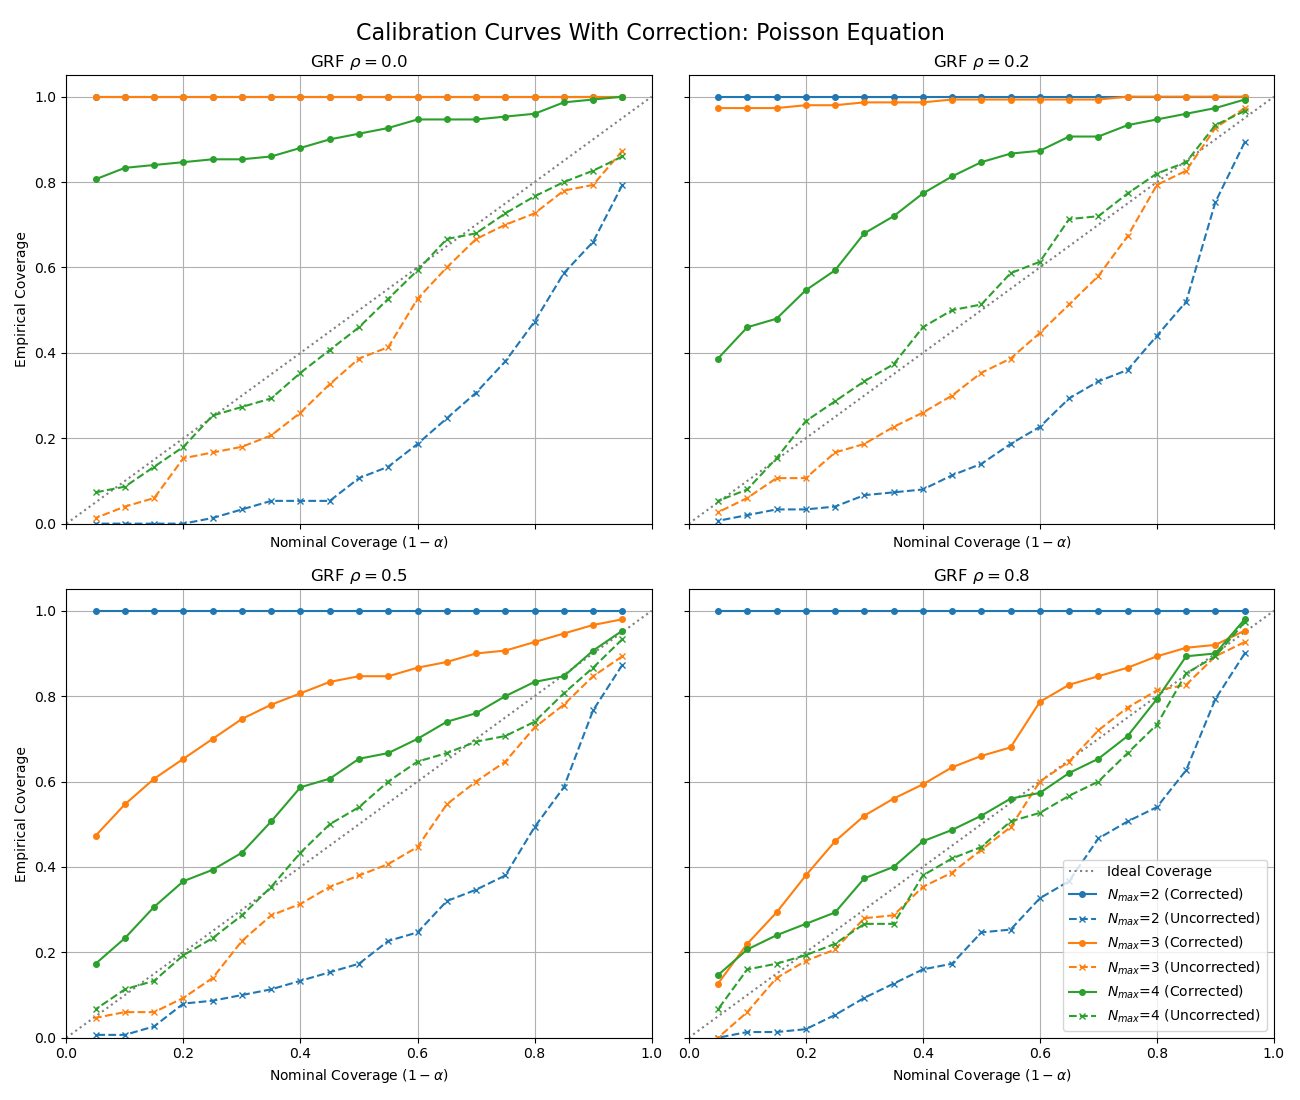
\includegraphics[width=\linewidth]{images/poisson_calibration.png}
\end{subfigure}
\begin{subfigure}{.45\textwidth}
  \centering
  \includegraphics[width=\linewidth]{images/rayleigh_calibration.png}
\end{subfigure}
  \caption{\label{fig:calibration} Calibration curves for conformal prediction regions over varying choices of Sobolev norm. Error bars across 10 trials are shown.}
\end{figure}

% To study this, we assume for the PDEs of interest herein, there is a truncation point $K^{*}$ sufficiently large that functions truncated at $K^{*}$ represent the ``true'' functions. It is further assumed that such a $K^{*}$ is larger than the ultimately observed truncation point $K$ and that generating data with the $K^{*}$ truncation is more expensive than can be feasibly run within the computational budget. Under such an assumption, computing $\widehat{q}_{\gamma}^{*}$ amounts to computing the quantile on this idealized dataset. 

% We first require empirical justification for the selection of $\gamma$, discussed in \Cref{section:gamma_selection}. Using such a selection, we then proceed in \Cref{section:experiments_pdebench} to study the optimization results across a number of PDE benchmark tasks from  \cite{takamoto2022pdebench}. While not semantically meaningful, performance of the procedure across such tasks demonstrates the versatility of the framework across PDEs. We then study the resulting downstream consequences in an application of interest, namely for emergency disaster relief for flooding \Cref{section:experiments_disaster}. Details are provided in \Cref{section:exp_details}, and code will be made public upon acceptance. 

% We first study FPO against a number of PDE benchmark tasks in \Cref{section:experiments_pdebench} to demonstrate the versatility of this approach across such use cases, namely the 2D Diffusion-Reaction equation, 2D Darcy Flow, and 2D shallow-water equations of \cite{takamoto2022pdebench}.
% In particular, we show the validity of the procedure across several PDE benchmark tasks from \cite{takamoto2022pdebench} in \Cref{section:experiments_pdebench_cov}, empirically verifying the claims on coverage made previously. We specifically demonstrate results across both the basic (the 1D advection/Burgers/Diffusion-Reaction/Diffusion-Sorption equations, 2D Diffusion-Reaction equation, and 2D Darcy Flow) and advanced (Compressible and incompressible Navier-Stokes equations and shallow-water equations) tasks. 

% \subsection{$\gamma$ Selection}\label{section:gamma_selection}
% In selecting $\gamma$, we wish to balanced two competing objectives: the ability to estimate $\widehat{q}_{\gamma}^{*}$ from finitely truncated data and the size of the resulting prediction region $\mathcal{C}_{\gamma}^{*}(a)$. As suggested by the result of \Cref{thm:func_cov}, the ability to estimate $\widehat{q}_{\gamma}^{*}$ improves with increasing $\gamma$. While this implication is informed from an inequality result in \Cref{thm:func_cov}, intuition naturally suggests the same trend, since higher-order norms, i.e. those for lower $\gamma$, are more sensitive to higher-order modes, rendering estimation with a finite truncation, in which such modes remain unobserved, harder in those cases. 

% As for the latter goal, the result of \Cref{lemma:suboptimality_guarantee} and typical intuitions of robust optimization suggest that the optimal adversarial perturbation set should achieve desired guarantees with minimal volume to minimize conservatism. We, therefore, seek to study the hypervolume $\mathrm{Vol}(\mathcal{C}_{\gamma}^{*}(a))$ as a function of $\gamma$. Notably, we are studying the \textit{idealized} prediction region volumes, i.e. under the true $\widehat{q}_{\gamma}^{*}$ rather than the truncated estimate $\widehat{q}_{\gamma}$. This is desired, as, if for instance $\mathcal{C}_{\gamma}^{*}(a)$ increases monotonically with $\gamma$, it then motivates the selection of $\gamma$ to be as small as possible such that $\widehat{q}_{\gamma}^{*}$ can be reasonably estimated with truncated data.

% To study this, we assume for the PDEs of interest herein, there is a truncation point $K^{*}$ sufficiently large that functions truncated at $K^{*}$ represent the ``true'' functions. It is further assumed that such a $K^{*}$ is larger than the ultimately observed truncation point $K$ and that generating data with the $K^{*}$ truncation is more expensive than can be feasibly run within the computational budget. Under such an assumption, computing $\widehat{q}_{\gamma}^{*}$ amounts to computing the quantile on this idealized dataset. 

% To then estimate the $\mathrm{Vol}(\mathcal{C}_{\gamma}^{*}(a))$, we note first that the Sobolev ball under finite truncation can be expressed as a quadratic form, namely $\mathcal{C}_{\gamma}^{*}(a) = \{\vec{u} : (\mathcal{G}(a) - \vec{u})^{\top} \mathcal{K} (\mathcal{G}(a) - \vec{u})\le\widehat{q}_{\gamma}^{*}\}$, where $\vec{u}\in\mathbb{R}^{(K^{*})^{d}}$ is a flattened representation of the modes and $\mathcal{K}$ contains the appropriate Sobolev norm scaling factors. For instance, if $\widetilde{\vec{u}}\in\mathbb{R}^{K^{*}\times K^{*}}$, we flatten the modes as $\vec{u}_{k_{1}K^{*} + k_{2}} = \widetilde{\vec{u}}_{k_{1},k_{2}}$ with the weighting matrix being $\mathcal{K}_{k_{1},k_{2}} = (1 + (k_{1} + k_{2})^{2\cdot2})^{s-\gamma}$. From here, we can estimate the hypervolume using Stirling's approximation for the volume of an $n$-ball. As we only wish to study this as a function of $\gamma$, we can ignore constants that do not vary with $\gamma$, leaving
% \begin{equation}\label{eqn:region_volume}
%     \mathrm{Vol}(\mathcal{C}_{\gamma}^{*}(a))
%     % \approx \left(\frac{1}{\sqrt{\pi (K^{*})^{d}}}\right) \left(\frac{2\pi e}{(K^{*})^{d}}\right)^{(K^{*})^{d} / 2} 
%     \propto \sqrt{(\widehat{q}_{\gamma}^{*})^{(K^{*})^{d}}
%     \det\left(\mathcal{K}^{-1}\right)}
%     = \sqrt{\frac{(\widehat{q}_{\gamma}^{*})^{(K^{*})^{d}}}{\prod_{k\in\mathbb{Z}^{d} : | k |_{\infty} \le K} (1 + || k ||_{1}^{2d})^{s-\gamma}}
%      }
% \end{equation}
% We now study this growth over a number of PDEs. In particular, we consider the following PDEs under doubly periodic boundary conditions:
% \begin{gather}
%     \mathrm{Poisson:}\qquad \nabla^{2} u = f \quad x\in(0,2\pi)^{d} \qquad u = 0\quad x\in\partial(0,2\pi)^{d} \\
%     \mathrm{Rayleigh–Benard:}\qquad \nabla^{2} u = f \quad x\in(0,2\pi)^{d} \qquad u = 0\quad x\in\partial(0,2\pi)^{d} 
% \end{gather}
% For such PDEs, we generated spectral pairs using the Dedalus spectral solver \cite{burns2020dedalus}, specifically taking $d=2$. For each PDE, a complete dataset of 1,000 i.i.d. data points was generated, with 750 reserved for training the spectral operator and the remaining 250 for calibration and testing. For each experiment, we present results with error bars across 10 trials, with trials differing in their sampling of points from the 250 held-out points used for calibration. In particular, 150 points were drawn from the 250 to create the calibration set and 100 for assessment, used in subsequent sections. $K^{*}$ was taken to be 256 in these experiments. Fixing $\alpha = 0.05$, we then computed the volume per \Cref{eqn:region_volume}, shown in \Cref{fig:volume}. Note that, to avoid issues of overflow, we instead computed $\log(\mathrm{Vol}(\mathcal{C}_{\gamma}^{*}(a)))$.

% \begin{figure}[H]
%   \centering 
% \begin{subfigure}{.45\textwidth}
%   \centering
%   \includegraphics[width=\linewidth]{images/poisson_volume.png}
% \end{subfigure}
% \begin{subfigure}{.45\textwidth}
%   \centering
%   \includegraphics[width=\linewidth]{images/rayleigh_volume.png}
% \end{subfigure}
%   \caption{\label{fig:volume} Volume of the prediction regions as a function of the choice of Sobolev norm parameter $\gamma$. Error bars across 10 trials are also shown, though low variance across trials makes them difficult to see.}
% \end{figure}

% This consistent monotonic growth across PDEs over $\gamma$ suggests that lower $\gamma$ results in smaller prediction regions, in turn motivating the use of as small a $\gamma$ as can be well-estimated from finitely truncated data.

\subsection{Robust Decision Making}
We now leverage the robust optimization algorithm given in \Cref{alg:fpo} and compare the regrets of solving the continuous space maximal coverage problem across the nominal and robust specifications. We first provide verification of the gradient expression derived in \Cref{section:opt_alg}, namely by visualizing both the robust field $\widehat{J}_{\mathrm{rob}}$ and the optimization trajectory of $w$ from \Cref{alg:fpo}, where $\widehat{J}_{\mathrm{rob}}(w) := \max_{\{\widehat{u}_{k}\}\in\ell^{2}(\mathbb{C})} J[w, \{\widehat{u}_{k}\}]$ is computed for each point in the domain, computed in a manner identical to the corresponding step of \Cref{alg:fpo} via \Cref{thm:constrained_soln}. Note that, while we explicitly compute the entire field in these examples, practical solution of this optimization problem is still desirable via gradient-based optimization, hence why it remains the approach employed in our experiments. 

We, therefore, show the optimization trajectory for one of the experiment trials for both the Poisson and Navier Stokes setups in \Cref{fig:poisson_traj}. Additional examples of such optimization trajectories are provided in \Cref{section:addn_results}. These visualizations first reveal the qualitative nature of the robust field solution; recall that the nominal approach can be solved by convolving a circular filter $\mathcal{B}_{r}$ over the domain and finding the consequent maximal value. The robust solution, therefore, takes on a similar form but also hedges against the granular, higher-order mode details predicted in the nominal solution. Such visualizations additionally confirm the gradient expression of \Cref{eqn:grad} and the corresponding maximization from \Cref{thm:constrained_soln}.

\begin{figure}[H]
  \centering 
  \includegraphics[width=\linewidth]{images/poisson_fields_A.png}
  \includegraphics[width=\linewidth]{images/navier_stokes_fields_A.png}
  \caption{\label{fig:poisson_traj} The true and surrogate field predictions are depicted for one of the Poisson equation tasks in the top row, respectively in the left and middle panes. The right pane demonstrates appropriate convergence to the local optimum in the robust field. A similar depiction is provided in the bottom row of the Navier Stokes vorticity equation.}
\end{figure}

To assess the quantitative improvement in using the robust formulation, we compare the suboptimality gaps, as defined in \Cref{eqn:subopt_gap} of the nominal and robust formulations. To ensure comparability across samples, we further scale this quantity by the true optimal value per sample, that is, considering instead $\Delta_{\%}(a, u) := \Delta_{\gamma}(a, u) / \min_{w\in\mathcal{W}} J[w, u]$, where we do not explicitly retain $\gamma$ in the notation as it is fixed over the experiments. Such scaled suboptimality gaps were computed across 100 i.i.d. test samples over both tasks. For each task, a paired t-test was conducted to assess whether the robust formulation offered significant improvements over the nominal baselines, with the hypothesis
\begin{gather*}
    H_{0}:\Delta^{(\mathrm{rob})}_{\%} = \Delta^{(\mathrm{nom})}_{\%}
    \qquad
    H_{1}: \Delta^{(\mathrm{rob})}_{\%} < \Delta^{(\mathrm{nom})}_{\%}
\end{gather*}
Such hypotheses tests were conducted with an $\alpha=0.01$, not to be confused with the $\alpha$ used for quantile specification in the conformal procedure. The final results are given in \Cref{table:pred_opt_results}. As expected, the resulting misspecification in the prediction of $\widehat{\mathcal{G}}(\theta)$ results in suboptimal decision making in the nominal specification, which is accounted for by the robust FPO formulation, thus resulting in significant reductions in the suboptimality. 

\begin{table}[H]
\centering
\caption{\label{table:pred_opt_results} P-values of the paired t-tests comparing gap proportions ($\Delta_{\%}$) are shown, conducted over 100 i.i.d. test samples.}
\begin{tabular}[t]{cc}
\toprule
PDE & p-value: $\Delta^{(\mathrm{rob})}_{\%} = \Delta^{(\mathrm{nom})}_{\%}$ \\
\midrule
Poisson & $3.61\times10^{-4}$ \\
Navier Stokes & $9.50\times10^{-4}$\\
\bottomrule
\end{tabular}
\end{table}

% \subsection{Robust Storm Planning}\label{section:experiments_pdebench}
% Neural operators have recently been leveraged for natural disaster prediction, such as for hurricanes \cite{pathak2022fourcastnet}, landslides \cite{chen2024deep}, and flooding \cite{sun2023rapid}. We focus on the first of these, seeking here to find the optimal placement of optimal disaster relief sites. One approach to predict such storm scenarios was studied in \cite{asselin2020penetration}, in which the 2D QG-Near Inertial Wave (QG-NIW) equations were used for storm modeling, which was further extended in \cite{wagner2015available,wagner2016three}. The relevant governing equations are given by
% \begin{align*}
% q &= \nabla^2 \psi + \frac{1}{f} \left[ \frac{1}{4} |\nabla^2 \phi|^2 + \frac{i}{2} J(\phi^*, \phi) \right]; \\
% q_t &+ J(\psi, q) = 0; \\
% \phi_t &+ J(\psi, \phi) + \phi \frac{i}{2} \nabla^2 \psi - \frac{i}{2} \frac{N^2}{f m^2} \nabla^2 \phi = 0.
% \end{align*}
% We, therefore, follow the setup discussed in \Cref{section:gamma_selection}, except we here simply fix $\gamma = 2 - \epsilon$ and do not reserve a subset of the calibration points for evaluation. We then leverage the robust optimization algorithm given in \Cref{alg:fpo} and compare the regrets of solving the continuous space maximal coverage problem across the nominal and robust specifications. The final results are given in \Cref{table:disaster_results}. As expected, the resulting misspecification in the prediction of $\widehat{\mathcal{G}}(\theta)$ results in suboptimal decision making in the nominal specification, which is accounted for by the robust FPO formulation.

% \subsection{Disaster Relief}\label{section:experiments_disaster}

% \begin{table}[H]
% \caption{\label{table:disaster_results} Median regret over 1,000 i.i.d. test samples with median absolute deviations in parentheses. 
% }
% \centering
% % \resizebox{\columnwidth}{!}{%
% \begin{tabular}[t]{cc}
% \toprule
% Nominal & FPO \\
% \midrule
% 1 & 0 \\
% \bottomrule
% \end{tabular}
% % }
% \end{table}

% Neural operators have recently been leveraged in scientific problems of interest, such as weather prediction \cite{pathak2022fourcastnet} and carbon plume modeling \cite{wen2022accelerating}. We focus on the latter herein, in which the pressure buildup in carbon capture storage reservoirs was of interest. This initial work demonstrated how neural operators enable sufficient speedup as to allow for probabilistic assessment of storage pressures, from which informed decisions on injection design could be made \cite{nghiem2009simulation, zhang2012numerical,pacala2018negative}. Such probabilistic modeling, however, has no upstream coverage guarantees, diminishing the supposed robustness claim. We, therefore, now demonstrate how MFCP enables efficient robust injection design.  

\section{Discussion}\label{section:discussion}
We have presented an approach of leveraging conformal prediction over neural operator surrogates to define a robust shape optimization problem and demonstrated how to efficiently solve such a problem. This work suggests many directions for extension. The most immediate would be in extending this work to the ``optimize-then-discretize'' framework of shape optimization, in which a functional representation of $\mathbb{T}^{d}$ is used in place of its discretized counterpart. In addition, extending this work to enable more general topological design optimization, in which optimization iterates are permitted to modify topological properties of the design, would be of interest. Further, an exciting application direction would be scaling this pipeline to more extensive engineering design tasks.

\newpage
\section*{Acknowledgments}
We would like to acknowledge the assistance of volunteers in putting
together this example manuscript and supplement.

\appendix
\section{Sobolev Norm Bound Example}\label{section:bounded_norm_setup}
We provide an example of a setup where a Sobolev norm bound can be provided from the PDE problem formulation, as given on page 323 of \cite{evans2022partial}. We denote
\begin{equation}
    L u = -\sum_{i,j=1}^n \left( a^{ij}(x) u_{x_i} \right)_{x_j} + \sum_{i=1}^n b^i(x) u_{x_i} + c(x) u.
\end{equation}

\begin{theorem}
    Let $s$ be a nonnegative integer, and assume $a^{ij}, b^{i}, c \in C^{s+1}(\overline{\mathbb{T}^{d}}) \quad (i, j = 1, \ldots, n)$ and $f \in \mathcal{H}^{s}(\mathbb{T}^{d})$. Suppose that $u \in \mathcal{H}^{1}_{0}(\mathbb{T}^{d})$ is a weak solution of the boundary-value problem
    \begin{align}\label{eqn:sobolev_bound_setup}
        \begin{cases}
            Lu = f & \text{in } \mathbb{T}^{d} \\
            u = 0 & \text{on } \partial \mathbb{T}^{d}.
        \end{cases}
    \end{align}
    Assume finally $\partial \mathbb{T}^{d} \text{ is } C^{s+2}.$
    Then $u \in \mathcal{H}^{s+2}(\mathbb{T}^{d}),$ and we have the estimate
    \begin{align}\label{eqn:sobolev_bound}
        \|u\|_{\mathcal{H}^{s+2}(\mathbb{T}^{d})} \leq C \left( \|f\|_{\mathcal{H}^{s}(\mathbb{T}^{d})} + \|u\|_{L^{2}(\mathbb{T}^{d})} \right),
    \end{align}
    the constant $C$ depending only on $s$, $\mathbb{T}^{d}$ and the coefficients of $L$. If $u$ is further the unique solution of \Cref{eqn:sobolev_bound_setup}, then estimate \Cref{eqn:sobolev_bound} simplifies to read
    \begin{align}
        \|u\|_{\mathcal{H}^{s+2}(\mathbb{T}^{d})} \leq C \|f\|_{\mathcal{H}^{s}(\mathbb{T}^{d})}.
    \end{align}
\end{theorem}

\section{Functional Coverage Guarantee}\label{section:coverage_guarantee}
\begin{theorem}
    Let $A^{(i)}\cup A'\overset{\mathrm{iid}}{\sim}\mathcal{P}(\mathbb{R}^{K^{d}})$ and $\mathcal{G} : \mathbb{R}^{K^{d}}\rightarrow(\mathbb{Z}^{d}\rightarrow\mathbb{R})$ such that $\mathcal{P}(\{U_{k}\}\mid a) = \delta(\mathcal{G}(a))$ and $\mathcal{P}_{A}(|| \mathcal{G}(A) ||_{s}\le B) = 1$. Further, let $\mathcal{D}_{C} := \{(a^{(i)}, \vec{u}^{(i)})\}$ with $\vec{u}^{(i)} := \{ u_{k} \}^{(i)}_{\le K}$. Let $\alpha\in(0,1)$ and $\widehat{q}_{\gamma}$ be the $\ceil{(N_{C}+1)(1-\alpha)}/N_{C}$ quantile of \Cref{eqn:score_func} over $\mathcal{D}_{C}$ for a fixed $\widehat{\mathcal{G}}$ and $\gamma\in\{1,...,s-1\}$. Then
    \begin{equation}
        \mathcal{P}_{A'}\left(\sum_{k\in\mathbb{Z}^{d}} (1 + || k ||_{1}^{2d})^{s-\gamma} ([\widehat{\mathcal{G}}(A')]_{k} - [\mathcal{G}(A')]_{k})^{2}
        \le \widehat{q}_{\gamma} + BK^{-2d\gamma} \right) \ge 1-\alpha.
    \end{equation}
\end{theorem}
\begin{proof}
    We consider the event of interest conditionally on the event $A' = a'$ such that $s(a', \{\mathcal{G}(a')\}_{\le K})\le\widehat{q}_{\gamma}$. Then:
    \begin{gather*}
         \sum_{k\in\mathbb{Z}^{d}} (1 + || k ||_{1}^{2d})^{s-\gamma} ([\widehat{\mathcal{G}}(a')]_{k} - [\mathcal{G}(a')]_{k})^{2}  \\
        = \underbrace{ \sum_{k\in\mathbb{Z}^{d} : | k |_{\infty} \le K} (1 + || k ||_{1}^{2d})^{s-\gamma} ([\widehat{\mathcal{G}}(a')]_{k} - \vec{u}'_{k})^{2}}_{\mathcal{E}_{\le K}} + \underbrace{ \sum_{k\in\mathbb{Z}^{d} : | k |_{\infty} > K} (1 + || k ||_{1}^{2d})^{s-\gamma} (\widehat{u}'_{k})^{2} }_{\mathcal{E}_{> K}}
    \end{gather*}
    We now demonstrate how each of the above two terms can be bounded. For the former, the result immediately follows in noting that $\mathcal{E}_{\le K}$ is precisely $s_{\gamma}(a', \vec{u}')$, from which we have $\mathcal{E}_{\le K}\le\widehat{q}_{\gamma}$ directly by assumption on $(a', \vec{u}')$. For the latter, we appeal to standard techniques for Fourier truncation analysis as follows
    \begin{align*}
         \sum_{k\in\mathbb{Z}^{d} : | k |_{\infty} > K} (1 + || k ||_{1}^{2d})^{s-\gamma} (\widehat{u}'_{k})^{2} 
        &=  \sum_{k\in\mathbb{Z}^{d} : | k |_{\infty} > K} \frac{(1 + || k ||_{1}^{2d})^{s}}{(1 + || k ||_{1}^{2d})^{\gamma}} (\widehat{u}'_{k})^{2}  \\
        &\le \frac{1}{(1 + K^{2d})^{\gamma}}  \sum_{k\in\mathbb{Z}^{d} : | k |_{\infty} > K} (1 + || k ||_{1}^{2d})^{s} (\widehat{u}'_{k})^{2}
        \le B K^{-2d\gamma}.
    \end{align*}
    We conclude by noting that $\mathcal{P}_{A'}(s(A', \{\mathcal{G}(A')\}_{\le K})\le\widehat{q}_{\gamma}) \ge 1 - \alpha$ from standard results of conformal prediction, completing the proof.  
\end{proof}

\section{Suboptimality Gap Lemma}\label{section:suboptimalty_gap}
% \begin{lemma}
%     Consider any $J[w, \{u_{k}\}]$ that is $L_{J}$-Lipschitz in $\{u_{k}\}$ under the metric $||\cdot||_{\mathcal{L}^{2}(\mathbb{T}^{d})}$ for any fixed $w$. Suppose $\mathcal{D}_C, A, \mathcal{G}, \alpha, \widehat{q}_{\gamma}, K$, and $B$ are defined as stated in \Cref{thm:func_cov}. Then
%     \begin{equation}
%         \mathcal{P}_{A}\left(0 \le \Delta_{\gamma}(A, \mathcal{G}(A)) \le L_{J} (\widehat{q}_{\gamma} + B K^{-2d\gamma})\right) \ge 1 - \alpha.
%     \end{equation}
% \end{lemma}
\begin{lemma}\label{lemma:suboptimality_guarantee}
    Consider any $J[w, u]$ that is $L_{J}$-Lipschitz in $u$ under the metric $||\cdot||_{\mathcal{L}^{2}(\mathbb{T}^{d})}$ for any fixed $w$. Suppose $\mathcal{D}_C, A, \mathcal{G}$, and $\alpha$ are defined as stated in \Cref{thm:func_cov} and $\widehat{\mathfrak{q}}_{\gamma}^{*}$ as in \Cref{eqn:real_space_region}. Then
    \begin{equation}
        \mathcal{P}_{A}\left(0 \le \Delta_{\gamma}(A, \mathcal{G}(A)) \le L_{J} \widehat{\mathfrak{q}}_{\gamma}^{*} \right) \ge 1 - \alpha.
    \end{equation}
\end{lemma}

\begin{proof}
    This follows immediately from related proofs in previous works, namely in \cite{patel2023conformal}. We again proceed by considering the event of interest conditionally on the event $A' = a'$ such that $\mathcal{G}(a')\in\mathfrak{C}_{\gamma}^{*}(a)$. Clearly then $\min_{w\in\mathcal{W}} \max_{\widehat{u}\in\mathfrak{C}_{\gamma}^{*}(a)} J[w, \widehat{u}] \ge \min_{w\in\mathcal{W}} J[w, u]$, since $u\in\mathfrak{C}_{\gamma}^{*}(a)$. For the upper bound, observe
    \begin{align*}
        \Delta_{\gamma}(A, \mathcal{G}(A))
        &:= \min_{w\in\mathcal{W}} \max_{\widehat{u}\in\mathfrak{C}_{\gamma}^{*}(a)} J[w, \widehat{u}] - \min_{w} J[w, u] \\
        &\le \max_{w\in\mathcal{W}} | \max_{\widehat{u} \in \mathfrak{C}_{\gamma}^{*}(a)} J[w, \widehat{u}] - J[w, u] | \\ 
        &\le L_{J} \max_{\widehat{u} \in \mathfrak{C}_{\gamma}^{*}(a)} || \widehat{u} - u ||_{\mathcal{L}^{2}(\mathbb{T}^{d})} \\
        &\le L_{J} \max_{\widehat{u} \in \mathfrak{C}_{\gamma}^{*}(a)} || \widehat{u} - u ||_{s-\gamma} 
        \le L_{J} \widehat{\mathfrak{q}}_{\gamma}^{*},
    \end{align*}
    where we use the standard fact that $|| f ||_{\mathcal{L}^{2}(\mathbb{T}^{d})}\le|| f ||_{s}$ for any $s$. We again conclude by leveraging that $\mathcal{P}_{A'}(\mathcal{G}(A')\in\mathfrak{C}_{\gamma}^{*}(A)) \ge 1 - \alpha$, completing the proof.
\end{proof}

\section{Generalized Danskin's Theorem}\label{section:gen_danskin}
We now proceed through the proof of the maximization gradient expression, which follows in demonstrating the conditions of the Generalized Danskin's Theorem are satisfied. The latter is replicated below for convenience.

\begin{theorem}\label{thm:gen_danskin}
    (Proposition A.13 from \cite{ulbrich2024generalized}) Assume the following:
    \begin{enumerate}
        \item $(W, ||\cdot||_{W})$ is a normed space, $\mathcal{W}\subset W$ is open, and $(W,\tau_{W})$ is a Haussdorf topological vector space with a topology $\tau_{W}$ such that the identity on $W$ is $|| \cdot ||_{W}$-$\tau_{W}$ continuous.
        \item $(U,\tau_{U})$ is a Hausdorff topological space.
        \item $\mathcal{U}\subset U$ is a sequentially compact set with respect to $\tau_{U}$.
        \item $J : \mathcal{W}\times \mathcal{U}\rightarrow\mathbb{R}$ is sequentially upper semicontinuous with respect to $\tau_{W}\times \tau_{\mathcal{U}}$ and $J(\cdot,u) : \mathcal{W}\rightarrow\mathbb{R}$ is sequentially continuous with respect to $\tau_{W}$ for all $u\in \mathcal{U}$.
        \item $J : \mathcal{W}\times \mathcal{U}\rightarrow\mathbb{R}$ is Fréchet differentiable in the first variable and $\partial_{w} J : \mathcal{W}\times \mathcal{U}\rightarrow W^{*}$ is sequentially continuous with respect to $\tau_{W}\times\tau_{U}$.
    \end{enumerate}
    Further assume the correspondence $M : W\rightarrow U$ defined by $M(w) := \{u : \max_{u\in\mathcal{U}} J[w, u] \}$ is single-valued on an $||\cdot ||$-open set $W_{X}\subset W$, then $J : W_{X}\rightarrow\mathbb{R}$ is Fréchet differentiable and $\partial_{w} \phi(w) = \partial_{w} J[w, M(w)]$.
    % Then $\phi : \mathcal{W}\rightarrow\mathbb{R}$ is Gâteaux differentiable at $w$ and there holds:
    % \begin{equation}
    %     \partial_{w} \phi(w,h) = \langle \partial_{w} J[w, \widehat{u}^{*}_{w}], h \rangle_{W^{*},W}.
    % \end{equation}
\end{theorem}

\begin{theorem}
    Let $\mathbb{R}^{d}$ be endowed with the topology $\tau_{W}$ induced by the standard Euclidean inner product $\langle \cdot,\cdot \rangle$ and similarly $\mathcal{L}^{2}(\mathbb{T}^{d})$ with the topology $\tau_{U}$ by the $\langle \cdot, \cdot \rangle_{ \mathcal{L}^{2}(\mathbb{T}^{d})}$. Let $J[w, u]$ be as defined in \Cref{eqn:collection_prob}, where $w\in(0,2\pi)^{d}$ and $u\in\mathcal{U}\subset\mathcal{L}^{2}(\mathbb{T}^{d})$ compact and strictly convex. Denote by $\phi(w) := \max_{\widehat{u}\in\mathcal{U}} J[w, \widehat{u}]$ and $\widehat{u}^{*}_{w} := \argmax_{\widehat{u}\in\mathcal{U}} J[w, \widehat{u}]$. Then $\phi(w)$ is Fréchet differentiable for any $w\in(0,2\pi)^{d}$ and $\partial_{w} \phi(w) = \partial_{w} J[w, \widehat{u}^{*}_{w}]$.
\end{theorem}
\begin{proof}
    The proof immediately follows in demonstrating the assumptions of \Cref{thm:gen_danskin} are satisfied in the setting of interest, as we do below.
    
    1. We have that $(\mathbb{R}^{d}, ||\cdot||_{\mathbb{R}^{d}})$ is a normed space by assumption. Further, $\mathcal{W} := (0,2\pi)^{d}$ is clearly open. $(\mathbb{R}^{d},\tau_{W})$ is a (finite-dimensional) Hilbert space and, therefore, a Haussdorf topological vector space.
    % By assumption, $w\in\mathbb{T}^{d}\subset\mathbb{R}^{d}$ (for either $d=2$ or $d=3$ in practice) is a normed subspace and with an openness assumption imposed by the statement of the optimization problem. 
    
    2. Similarly, $(\mathcal{L}^{2}(\mathbb{T}^{d}), \tau_{U})$ is a Hilbert space and, therefore, a Haussdorf topological vector space.
    
    3. Again, given that $(\mathcal{L}^{2}(\mathbb{T}^{d}), \tau_{U})$ is a metric space, a subset $\mathcal{U}$ is sequentially compact if and only if it is compact, which is true by assumption.
    
    4. We first demonstrate that $J[w, u]$ is sequentially upper semicontinuous with respect to $\tau_{W}\times\tau_{U}$. Clearly, the product space $\mathcal{W}\times\mathcal{U}$ is a metric space by the metric structure of the individual spaces $\mathcal{W}$ and $\mathcal{U}$. We, therefore, seek to demonstrate $J[w, u]$ is upper semicontinuous with respect to $\tau_{W}\times\tau_{U}$ as, over metric spaces, such a map $J[w, u]$ is sequentially continuous if and only if it is continuous. It then suffices to demonstrate that $J[w, u]$ is jointly continuous in $(w, u)$, as a function is continuous if and only if it is both upper and lower semi-continuous. To prove joint continuity, we leverage the following lemma.
    
    % To demonstrate sequential upper semicontinuity, we use the standard result that a function mapping between metric spaces $f : (X, d_{X})\rightarrow(Y, d_{Y})$ is sequentially continuous on $X$ if and only if it is continuous on $X$. Given that both spaces of interest have induced metric structure, it therefore suffices to demonstrate joint continuity in $(w,u)$. To prove this, we leverage the following lemma.

    \begin{lemma}\label{lemma:joint_cts}
        Let $\mathcal{X}$ be a metrizable topological space and $\mathcal{V}$ and $\mathcal{W}$ be Fréchet spaces. Then, any separately continuous map $\mathcal{X}\times \mathcal{V}\rightarrow \mathcal{W}$ that is linear in its second variable is jointly continuous.
    \end{lemma}
    \begin{proof}
        Denote by $f(x,v) : \mathcal{X}\times \mathcal{V}\rightarrow \mathcal{W}$ a function that is linear in $v$ and separately continuous, i.e. in $f(x_{0},\cdot)$ is continuous in $v$ for any fixed $x_{0}$ and similarly $f(\cdot, v_{0})$ in $x$ for any fixed $v_{0}$. By definition, such an $f$ is then jointly continuous at $(x_{0}, v_{0})$ if for each open neighborhood $W$ of $f(x_{0}, v_{0})$, there are open sets $X$ and $V$ such that $f(X\times V)\subset W$ with $(x_{0},v_{0})\in X\times V$. 
        
        To demonstrate this, consider some open neighborhood $W$ of $f(x_{0}, v_{0})$. We now leverage the separate continuity of $f$ in $x$ for a fixed $v_0$, in particular at the point $x=x_0$. By this, we have that, for the aforementioned neighborhood $W$ around $f(x_0, v_0)$, we have an open set $X_{v_0}$ such that $f(X_{v_0}, v_0) \subset W$ and $x\in X_{v_0}$. By the local compactness of $\mathcal{X}$, we further know that there is a compact set $K_{v_{0}}\subset X_{v_0}$ with $x\in K_{v_0}$ similarly with $f(K_{v_0}, v_0) \subset W$. Again by the continuity of $f(\cdot, v)$, we have that $f(K_{v_0}, v)$ is compact for any fixed $v\in\mathcal{V}$, further implying such a $f(K_{v_0}, v)$ is bounded for any $v\in\mathcal{V}$. 
        
        Consider now the subspace $H$ of linear functions, defined over fixed $x_0\in K_{v_0}$, i.e. $H := \{ f(x_0,\cdot) : x_0\in K_{v_0}\}$. We now leverage the linear structure of such maps using the following proposition. 

        \begin{proposition}
            (Proposition 11.1.1 from \cite{jarchow2012locally}) Hausdorff locally convex space $\mathcal{E}$ is barrelled if and only if for every Hausdorff locally convex space $\mathcal{F}$ any pointwise bounded subset of $\mathcal{L}(\mathcal{E}, \mathcal{F})$, namely the space of continuous linear maps from $\mathcal{E}$ into $\mathcal{F}$, is equicontinuous.
        \end{proposition}
    
        Since $\mathcal{V}$ is a Fréchet space by assumption, we immediately have that it is a barrelled space. Since $\mathcal{W}$ too is a Fréchet space, it is a Hausdorff locally convex space, from which we have that any pointwise bounded subset of $\mathcal{L}(\mathcal{V}, \mathcal{W})$ is equicontinuous. Notice that, by the previously discussed implications of the compactness of $K_{v_0}$, $H$ is pointwise bounded, i.e. for each $v\in\mathcal{V}$, from which we have that such a set is equicontinuous. By definition of equicontinuity, for the neighborhood $W$, there is some $V'\subset\mathcal{V}$ open with $v_{0}\in V'$ such that $f(K_{v_0}, V') \subset W$, completing the proof.
    \end{proof}

    % Such a lemma is immediately applicable as $X = \mathbb{R}^{d}$, $V = \mathcal{L}^{2}(\mathbb{T}^{d})$, and $W = \mathbb{R}$. 
    To see the predicates of such a lemma are satisfied, first note that $X := \mathbb{R}^{d}$ is metrizable under the Euclidean metric and $V = \mathcal{L}^{2}(\mathbb{T}^{d})$ and $W = \mathbb{R}$ are Hilbert and, hence, Fréchet spaces. In addition, $J(\cdot, u)$ is a linear functional, as:
    \begin{align*}
        J[w, \alpha u_{1} + \beta u_{2}]
        &:= \int_{\mathcal{B}_{r}(w)} (\alpha u_{1} + \beta u_{2})(x) dx \\
        &= \alpha \int_{\mathcal{B}_{r}(w)} u_{1}(x) dx + \beta \int_{\mathcal{B}_{r}(w)} u_{2}(x) dx
        = \alpha J[w, u_{1}] + \beta J[w, u_{2}].
    \end{align*} 
    Therefore, it suffices to demonstrate $J$ is separately continuous in $u$ and $w$ to conclude. For notational clarity, we re-express the functional as
    \begin{equation*}
        J[w, u] = \int_{\mathcal{B}_{r}(0)} u(x + w) dx.
    \end{equation*}
    Continuity in the first argument then immediately follows from the assumption that $u_{0}\in\mathcal{L}^{2}(\mathbb{T}^{d})$ for $\gamma\le s-1$. Again by the Sobolev embedding theorem, we have $\mathcal{H}^{s}(\mathbb{T}^{d})\subset\mathcal{C}^{0}(\mathbb{T}^{d})$
    Then, by the continuity of $u_{0}$ at any fixed $x_0\in(0,2\pi)^{d}$, for any $\epsilon >0$, there is some $\delta_{u_{0}}(\epsilon) > 0$ such that $|| x - x_{0} ||_{d} < \delta_{u_{0}}(\epsilon) \implies | u_{0}(x) - u_{0}(x_0) | < \epsilon$. To demonstrate the continuity of $J[\cdot, u_{0}]$ in $w$, consider any $\epsilon > 0$ and let $\delta := \delta_{u_{0}}(\epsilon / \mathrm{Vol}(\mathcal{B}_{r}(0)))$. Then, we have $|| w - w_0 || < \delta_{u_{0}}(\epsilon / \mathrm{Vol}(\mathcal{B}_{r}(0)))$ implies
    \begin{align*}
        | J[w, u_{0}] - J[w_{0}, u_{0}] |
        &:= \left| \int_{\mathcal{B}_{r}(0)} u_{0}(w + x) dx - \int_{\mathcal{B}_{r}(0)} u_{0}(w_{0} + x) dx \right| \\
        &\le \int_{\mathcal{B}_{r}(0)} \left|u_{0}(w + x) - u_{0}(w_{0} + x) \right| dx\\
        &\le \int_{\mathcal{B}_{r}(0)} \frac{\epsilon}{\mathrm{Vol}(\mathcal{B}_{r})} dx
        = \epsilon.
    \end{align*}    
    % thus implying such functions are continuously differentiable and, therefore, Lipschitz continuous. Denote by $L$ the Lipschitz constant for such a $u_{0}$, from which
    % Continuity in the first argument immediately follows from continuity of the integral of a continuous function. 
    % % That is, for any fixed $u_{0}$:
    % % \begin{gather*}
    % %     % \int_{\mathcal{B}_{r}} \left|u_{0}(w + x) - u_{0}(w_{0} + x)\right| dx
    % %     % \le \int_{\mathcal{B}_{r}} \epsilon / (2 \mathrm{Vol}(\mathcal{B}_{r})) dx
    % %     % \le \epsilon / 2.
    % % \end{gather*}
    % That is, by the continuity of $u_{0}$, we have that, for $x_{0}$ and $\epsilon > 0$, there is some $\delta_{U}(\epsilon, x_{0})$ such that $|| x - x_0 || < \delta_{U}(\epsilon, x_{0})\implies || u_{0}(x) - u_{0}(x_0) || < \epsilon$. Further note that, for any $w\in\mathcal{B}_{\delta}(w_{0})$ and $x\in\mathcal{B}_{r}$, we have that $w + x\in\mathcal{B}_{\delta + r}(w_{0})$. 
    % To now demonstrate the continuity of $J(\cdot, u_{0})$ for any fixed $u_{0}$, consider any $w_{0}\in\mathbb{R}^{d}$ and $\epsilon > 0$ and take $\delta :=  \min_{x\in\mathcal{B}_{\delta + r}(w_{0})} \delta_{U}(\epsilon / \mathrm{Vol}(\mathcal{B}_{r}), x)$. Then:
    % % for any fixed $u_{0}$, denote by $\delta_{W}(x)$ the condition for which $|| w - w_{0} || \le \delta_{W}(x) \implies | u_{0}(w + x) - u_{0}(w_{0} + x) | \le \epsilon / (2 \mathrm{Vol}(\mathcal{B}_{r}))$. Then, denoting $\delta_{W} := \min_{x\in\mathcal{B}_{r}} \delta_{W}(x)$, we have:
    % \begin{gather*}
    %     | J(w, u_{0}) - J(w_{0}, u_{0}) |
    %     := \left| \int_{\mathcal{B}_{r}} u_{0}(w + x) dx - \int_{\mathcal{B}_{r}} u_{0}(w_{0} + x) dx \right|
    %     \le \int_{\mathcal{B}_{r}} \left|u_{0}(w + x) - u_{0}(w_{0} + x) \right| dx 
    %     \le \int_{\mathcal{B}_{r}} \frac{\epsilon}{\mathrm{Vol}(\mathcal{B}_{r})} dx
    %     = \epsilon.
    % \end{gather*}
    % \begin{align*}
    %     % | u_{0}(w) - u_{0}(w_0) | \le L || w - w_0 ||_{2} \\
    %     | J[w, u_{0}] - J[w_{0}, u_{0}] |
    %     &:= \left| \int_{\mathcal{B}_{r}} u_{0}(w + x) dx - \int_{\mathcal{B}_{r}} u_{0}(w_{0} + x) dx \right| \\
    %     &\le \int_{\mathcal{B}_{r}} \left|u_{0}(w + x) - u_{0}(w_{0} + x) \right| dx\\
    %     &\le \int_{\mathcal{B}_{r}} L || (w + x) - (w_{0} + x) ||_{2}
    %     = L \mathrm{Vol}(\mathcal{B}_{r}) || w - w_{0} ||_{2}.
    % \end{align*}
    % This demonstrates that $J(\cdot, u_{0})$ is Lipschitz continuous with Lipschitz constant $L \mathrm{Vol}(\mathcal{B}_{r})$, from which the proof is complete as Lipschitz continuity implies continuity. 
    This also verifies the second subcondition of interest, namely that $J(\cdot,u) : \mathcal{W}\rightarrow\mathbb{R}$ is sequentially continuous with respect to $\tau_{W}$ for all $u\in \mathcal{U}$. To see separate continuity in the second argument, we then fix some $w_0$ and appeal to the fact that a linear functional is continuous if and only if it is bounded, which follows immediately as $\mathcal{L}^{p}(\mathbb{T}^{d})\subset\mathcal{L}^{q}(\mathbb{T}^{d})$ for any $1 \le p \le q \le \infty$. In particular, for $p = 2$ and $q = 1$, we know $u\in\mathcal{L}^{2}(\mathbb{T}^{d})\implies u\in\mathcal{L}^{2}(\mathbb{T}^{d})\implies u\in\mathcal{L}^{1}(\mathbb{T}^{d})$, from which we have:
    \begin{gather*}
        | J[w_0, u] |
        := \left| \int_{\mathcal{B}_{r}(w_0)} u(x) dx \right|
        \le \int_{\mathcal{B}_{r}(w_0)} \left| u(x) \right| dx
        \le \int_{\mathbb{T}^{d}} \left| u(x) \right| dx
        =: || u ||_{\mathcal{L}^{1}(\mathbb{T}^{d})} < \infty,
    \end{gather*}
    thereby completing the proof. 
    
    5. By the restriction of $d\in\{1,2,3\}$, Fréchet differentiability in the first variable follows immediately from the Leibniz integral rule (Reynolds transport theorem). In particular, $\partial_{w} J := \{\partial_{w_{i}} J[w, u]\}_{i=1}^{d}$, where the components are given by
    \begin{equation}\label{eqn:component_partial}
        \partial_{w_i} \int_{\mathcal{B}_{r}(w)} u(x) dx
        = \int_{\partial\mathcal{B}_{r}(w)} u(x)(v(w_i)\cdot\textbf{n}(x)) dx
        = \int_{\partial\mathcal{B}_{r}(w)} u(x)(e_i\cdot\textbf{n}(x)) dx,
    \end{equation}
    where $\partial\mathcal{B}_{r}(w)$ represents the surface boundary of $\mathcal{B}_{r}(w)$, $v(w_i)$ the surface boundary velocity, and $\textbf{n}(x)$ the surface normal of $\mathcal{B}_{r}(w)$. Notably, since the surface transport $\partial_{w_i}$ is axis-aligned, we have $v(w_i) = e_i$, where $e_i$ is the unit vector along coordinate $i$. Note that the non-boundary term of the Leibniz integral rule vanishes by the lack of dependence of $u(x)$ on $w$. 
    
    We now seek to demonstrate the map $\partial_{w} J$ is continuous with respect to $\tau_{W}\times\tau_{U}$. By classical results of multivariate calculus, continuity of $\partial_{w} J$ holds if and only if continuity holds for each component $\partial_{w_{i}} J[w, u]$. By the symmetry of \Cref{eqn:component_partial} in $i$, it therefore suffices to demonstrate joint continuity of $\partial_{w_{i}} J[w, u]$ for a fixed $i$. We now again appeal to \Cref{lemma:joint_cts} to demonstrate joint continuity via separate continuity in $u$ and $w$. This lemma remains applicable by the clear linearity of the above expression. 
    % The proof of this property follows in the same manner as that of the previous property, namely by demonstrating separate continuity and appealing to the result of \Cref{lemma:joint_cts}. Explicitly writing the gradient expression, we have
    % \begin{gather*}
    %     \partial_{w} J[w, u]
    %     := \partial_{w} \int_{\mathcal{B}_{r}} u(w + x) dx
    %     = \int_{\mathcal{B}_{r}} \partial_{w} u(w + x) dx.
    % \end{gather*}
    % In this case, $X := \mathbb{R}^{d}$, again metrizable under the Euclidean metric, and $V = \mathcal{L}^{2}(\mathbb{T}^{d})$ and $W = \mathbb{R}^{d}$, both of which are Fréchet spaces. In addition, $J(\cdot, u)$ remains a linear functional by linearity of the gradient:
    % \begin{gather*}
    %     \partial_{w} J[w, \alpha u_{1} + \beta u_{2}]
    %     := \int_{\mathcal{B}_{r}} \partial_{w} (\alpha u_{1} + \beta u_{2})(w + x) dx \\
    %     = \alpha \int_{\mathcal{B}_{r}} \partial_{w} u_{1}(w + x) dx + \beta \int_{\mathcal{B}_{r}} \partial_{w} u_{2}(w + x) dx
    %     = \alpha \partial_{w} J[w, u_{1}] + \beta \partial_{w} J[w, u_{2}].
    % \end{gather*} 
    
    To demonstrate separate continuity, we follow the proof strategy leveraged previously, namely rewriting \Cref{eqn:component_partial} as
    \begin{equation*}
        \partial_{w_i} J[w, u] 
        = \int_{\partial\mathcal{B}_{r}(0)} u(x+w)(e_i\cdot\textbf{n}(x)) dx
    \end{equation*}
    Observe that the proofs of separate continuity follow in exactly the previous manner. For $w$, consider some fixed $u_{0}$. Again, by the continuity of $u_{0}$ at any fixed $x_0\in(0,2\pi)^{d}$, for any $\epsilon >0$, there is some $\delta_{u_{0}}(\epsilon) > 0$ such that $|| x - x_{0} ||_{d} < \delta_{u_{0}}(\epsilon) \implies | u_{0}(x) - u_{0}(x_0) | < \epsilon$. To demonstrate the continuity of $\partial_{w_i} J[\cdot, u_{0}]$ in $w$, consider any $\epsilon > 0$ and let $\delta := \delta_{u_{0}}(\epsilon / \mathrm{Vol}(\partial\mathcal{B}_{r}(0)))$. Then, we have $|| w - w_0 || < \delta_{u_{0}}(\epsilon / \mathrm{Vol}(\partial\mathcal{B}_{r}(0)))$ implies
    \begin{align*}
        | \partial_{w_i} J[w, u_{0}] - \partial_{w_i} J[w_{0}, u_{0}] |
        &:= \left| \int_{\partial\mathcal{B}_{r}(0)} u(x+w)(e_i\cdot\textbf{n}(x)) dx - \int_{\partial\mathcal{B}_{r}(0)} u(x+w_{0})(e_i\cdot\textbf{n}(x)) dx \right| \\
        &\le \int_{\partial\mathcal{B}_{r}(0)} \left|u_{0}(w + x) - u_{0}(w_{0} + x) \right| | (e_i\cdot\textbf{n}(x)) | dx\\
        &\le \int_{\partial\mathcal{B}_{r}(0)} \frac{\epsilon}{\mathrm{Vol}(\partial\mathcal{B}_{r})} dx
        = \epsilon.
    \end{align*}
    For the second argument, we again demonstrate continuity by demonstrating boundedness, as linearity in $u$ remains for each component $\partial_{w_i} J[w, u]$. Boundedness follows as
    \begin{gather*}
        | \partial_{w_i} J[w, u] |
        := \left| \int_{\partial\mathcal{B}_{r}(0)} u(x+w)(e_i\cdot\textbf{n}(x)) \right|
        \le \int_{\partial\mathcal{B}_{r}(0)} \left| u(x) \right| dx 
        % \\
        % &\le \int_{\mathbb{T}^{d}} \left| u(x) \right| dx
        \le || u ||_{\mathcal{L}^{1}(\mathbb{T}^{d})} < \infty.
    \end{gather*}
    % \begin{gather*}
    %     || \partial_{w} J[w, u] ||_{2}
    %     := \left|\left| \int_{\partial\mathcal{B}_{r}(w)} (u(x)\cdot\textbf{n}) dx \right|\right|_{2}
    %     \le \int_{\partial\mathcal{B}_{r}(w)} \left|\left| u(x)\cdot\textbf{n} \right|\right|_{2} dx
    %     \le M_{\nabla} \mathrm{Vol}(\mathcal{B}_{r}),
    %     % := \left|\left| \int_{\mathcal{B}_{r}} \partial_{w} u(w + x) dx \right|\right|_{2}
    %     % \le \int_{\mathcal{B}_{r}} \left|\left| \partial_{w} u(w + x) \right|\right|_{2} dx
    %     % \le M_{\nabla} \mathrm{Vol}(\mathcal{B}_{r}),
    % \end{gather*}
    % where similarly $M_{\nabla} := \max_{w\in\mathbb{T}^{d}} M_{\nabla}(w) < \infty$ and $M_{\nabla}(w) := \max_{x\in\mathcal{B}_{r}(w)} || \nabla_{x} u(x) ||_{2} < \infty$ exists by the Lipschitz continuity of $\nabla_{x} u$ as argued above.
    We conclude by demonstrating $M(w) := \{u : \max_{u\in\mathcal{U}} J[w, u] \}$ is single-valued for any $w\in(0,2\pi)^{d}$. This immediately follows as any linear functional has a unique maximizer on a strictly convex set. Suppose we had $u\neq \widehat{u}^{*}_{w}$ such that $J[w, u] = J[w, \widehat{u}^{*}_{w}]$. By the strict convexity of $\mathcal{U}$, this would imply $u' := 1/2 (u + \widehat{u}^{*}_{w})$ lies in the interior of $\mathcal{U}$. We then denote by $u_{\epsilon}$ the constant function $u_{\epsilon}(x) := \epsilon$ $\forall x\in(0,2\pi)^{d}$. Since $u'$ lies in the interior of $\mathcal{U}$, there exists some $\epsilon > 0$ such that $u_{\epsilon}' := u' + u_{\epsilon}\in\mathcal{U}$, further implying
    \begin{gather*}
        J[w, u_{\epsilon}']
        := J[w, \frac{1}{2} (u + \widehat{u}^{*}_{w}) + u_{\epsilon}]\\
        = \frac{1}{2} (J[w, u] + J[w, \widehat{u}^{*}_{w}] + J[w, u_{\epsilon}])
        = J[w, \widehat{u}^{*}_{w}] + \frac{1}{2} J[w, u_{\epsilon}] > J[w, \widehat{u}^{*}_{w}],
    \end{gather*}
    contradicting the assumed maximization achieved by $\widehat{u}^{*}_{w}$, completing the proof.

%     \begin{lemma}\label{lemma:unique_max}
%         % Let $w\in(0,2\pi)^{d}$, $u\in\mathbb{R}^{K^{d}}$, and $u_{\le}^{*}(w, \vec{u})$ be as given by \Cref{eqn:max_subproblem}. Then, for any $u\in\mathcal{L}^{2}(\mathbb{T}^{d})\neq u_{\le}^{*}(w, \vec{u})$ such that $|| u - u_{\theta} ||_{s}\le\widehat{q}$, $J[w, u] < J[w, u_{\le}^{*}(w, \vec{u})]$.
%         Let $J[w, u]$ be as defined in \Cref{eqn:collection_prob}, where $w\in(0,2\pi)^{d}$ and $u\in\mathcal{U}\subset\mathcal{L}^{2}(\mathbb{T}^{d})$ compact. Then, for any $u\in\mathcal{U}\neq \widehat{u}^{*}_{w}$, $J[w, \widehat{u}^{*}] < J[w, u]$.
%     \end{lemma}
%     \begin{proof}
        
% \phantom\qedhere
%     \end{proof}
\end{proof}

\section{Linear Functional Robust Equivalence}\label{section:lin_robust}
We now consider a generalized form of the ``collection problem'' studied herein and demonstrate that, in the special case of considering a \textit{linear} functional that is a shift of an underlying ``template functional,'' the solutions to the nominal and robust solutions are identical. 

\begin{remark}
    Let $J[w, u] : (0,2\pi)^{d}\times\mathcal{L}^{2}(\mathbb{T}^{d})\rightarrow\mathbb{R}$ be a functional linear in $u$ whose dependence on $w$ is through a shift of a template functional $L : \mathcal{L}^{2}(\mathbb{T}^{d})\rightarrow\mathbb{R}$, i.e. $J[w, u] = L[u(\cdot-w)]$. Then, for any $u\in\mathcal{L}^{2}(\mathbb{T}^{d})$ and$s\in\mathbb{N}$, $w_{\mathrm{nom}}^{*}(u) = w_{\mathrm{rob}}^{*}(u)$, where
    \begin{equation*}
        w_{\mathrm{nom}}^{*}(u) := \argmin_{w\in(0,2\pi)^{d}} J[w, u]
        \qquad w_{\mathrm{rob}}^{*}(u) := \argmin_{w\in(0,2\pi)^{d}} \max_{\widehat{u}\in\mathcal{B}^{||\cdot||_{s}}_{\widehat{q}}[u]} J[w, u]
    \end{equation*}
\end{remark}
\begin{proof}
    By the Riesz representation theorem, for any $w\in(0,2\pi)^{d}$, there is a unique representer $\psi^{(w)}$ such that $J[w, \widehat{u}] = \langle \widehat{u}, \psi^{(w)} \rangle_{s}$. By the assumption that $J[w, u] = L[u(\cdot-w)]$ for some $L$, we have that such representers must similarly have the form $\psi^{(w)}(x) = \psi^{(0)}(x-w)$. Further, we note that, for any $\widehat{u}\in\mathcal{B}^{||\cdot||_{s}}_{\widehat{q}}[u]$, $\widehat{u} = u + v$, where $||v||_{s}\le\widehat{q}$. From this, we have
    \begin{align*}
        \max_{\widehat{u}\in\mathcal{B}^{||\cdot||_{s}}_{\widehat{q}}[\widehat{u]}} J[w, u]
        &= \max_{\widehat{u}\in\mathcal{B}^{||\cdot||_{s}}_{\widehat{q}}[\widehat{u]}} \langle \widehat{u}, \psi^{(0)}(x-w) \rangle \\
        &= \max_{v : ||v||_{s}\le\widehat{q}} \langle u + v, \psi^{(0)}(x-w) \rangle \\
        &= \langle u, \psi^{(0)}(x-w) \rangle + \max_{v : ||v||_{s}\le\widehat{q}} \langle v, \psi^{(0)}(x-w) \rangle \\
        &= J[w, u] + \widehat{q} \max_{v : ||v||_{s}\le 1} \langle v, \psi^{(0)}(x-w) \rangle
        =: J[w, u] + \widehat{q} || \psi^{(0)}(x-w) ||_{s^{*}},
    \end{align*}
    where $|| \cdot ||_{s^{*}}$ denotes the dual $s$-Sobolev norm, which follows directly from the definition. Notably, the Sobolev $s$-norm is shift invariant over $\mathbb{T}^{d}$, as Fourier coefficients only change by a phase upon a shift of the underlying function. That is, since $\widehat{\phi}^{(w)}_{k} = e^{-2\pi i k w} \widehat{\phi}^{(0)}_{k}$, $| \widehat{\phi}^{(w)}_{k} | = | \widehat{\phi}^{(0)}_{k} |$, from which we have that:
    \begin{align*}
        || \phi^{(w)} ||^{2}_{s}
        &:= \sum_{k\in\mathbb{Z}^{d} : | k |_{\infty} \le K} (1 + || k ||_{1}^{2d})^{s} (\widehat{\phi}^{(w)}_{k})^{2} \\
        &= \sum_{k\in\mathbb{Z}^{d} : | k |_{\infty} \le K} (1 + || k ||_{1}^{2d})^{s} (\widehat{\phi}^{(0)}_{k})^{2}
        =: || \phi^{(0)} ||^{2}_{s}
    \end{align*}
    Given the shift invariance of $|| \cdot ||_{s}$, it immediately follows that the dual $|| \cdot ||_{s^{*}}$ too is shift invariant, which can be seen as follows. Denote by $T_{w} : \mathcal{L}^{2}(\mathbb{T}^{d})\rightarrow\mathcal{L}^{2}(\mathbb{T}^{d})$ the shift by $w$ operator, i.e. $T_{w}(f(x)) := f(x-w)$, for which the adjoint $T^{*}_{w} = T_{-w}$. With this,
    \begin{align*}
        || \psi^{(0)}(x-w) ||_{s^{*}}
        &:= \max_{v : ||v||_{s}\le 1} \langle v, \psi^{(0)}(x-w) \rangle \\
        &= \max_{v : ||v||_{s}\le 1} \langle v, T_{w}(\psi^{(0)}(x)) \rangle \\
        &= \max_{v : ||v||_{s}\le 1} \langle T_{-w} (v), \psi^{(0)}(x) \rangle \\ 
        &= \max_{v : ||T_{-w} (v)||_{s}\le 1} \langle T_{-w} (v), \psi^{(0)}(x) \rangle \qquad \text{by translation invariance of } || \cdot ||_{s} \\ 
        &= \max_{\widetilde{v} : ||\widetilde{v}||_{s}\le 1} \langle \widetilde{v}, \psi^{(0)}(x) \rangle =: || \psi^{(0)}(x) ||_{s^{*}}
    \end{align*}
    For any $w$, therefore, $\max_{\widehat{u}\in\mathcal{B}^{||\cdot||_{s}}_{\widehat{q}}[\widehat{u]}} J[w, u] = J[w, u] + \widehat{q} || \psi^{(0)}(x) ||_{s^{*}}$ is constant over $w$. Thus,
    \begin{align*}
        w_{\mathrm{rob}}^{*}(u) := \argmin_{w\in(0,2\pi)^{d}} \max_{\widehat{u}\in\mathcal{B}^{||\cdot||_{s}}_{\widehat{q}}[u]} J[w, u]
        &:= \argmin_{w\in(0,2\pi)^{d}} \left(J[w, u] + \widehat{q} || \psi^{(0)}(x) ||_{s^{*}} \right)\\
        &= \argmin_{w\in(0,2\pi)^{d}} J[w, u]
        =: w_{\mathrm{nom}}^{*}(u).
    \end{align*}
\end{proof}

\section{Maximization Subproblem}\label{section:maximizer_pf}
% \begin{theorem}
%     Suppose $\widehat{\mathcal{G}}$ and $\gamma$ are defined as in \Cref{thm:func_cov}; $\widehat{q}_{\gamma}^{*}$ as in \Cref{section:func_score}; and $\widehat{u}^{*}_{w}$ as in \Cref{eqn:max_subproblem} for some fixed $a\in\mathbb{R}^{K^{d}}$ and $w\in(0,2\pi)^{d}$. Assume $\widehat{q}_{\gamma}^{*} > 0$. Then, $\widehat{u}^{*}_{w} = \sum_{k\in\mathbb{Z}^{d}} \widehat{u}^{*}_{k} \phi_{k}(x)$, where
%     \begin{equation}
%         \widehat{u}^{*}_{k} = [\widehat{\mathcal{G}}(a)]_{k} + \frac{\widehat{q}_{\gamma}^{*}}{|| \Phi^{(w)} ||_{s-\gamma}} \frac{\Phi^{(w)}_k}{(1 + || k ||_{1}^{2d})^{s-\gamma}} 
%     \end{equation}
%     where $\Phi_{k}^{(w)} := \int_{\mathcal{B}_{r}(w)} \phi_{k}(x) dx$ and $\Phi^{(w)} := \sum_{k\in\mathbb{Z}^{d}} (1 + || k ||^{2d}_{1})^{-(s-\gamma)} \overline{\Phi_{k}^{(w)}}$.
% \end{theorem}
% \begin{proof}
% As stated in the main text, computing this maximizer follows in noting that there is a unique representer $\psi$ such that $J[w, \widehat{u}] = \langle \widehat{u}, \psi\rangle_{s-\gamma}$. Notably, any $\widehat{u}\in\mathfrak{C}_{\gamma}^{*}(a)$ can be expressed as $\widehat{u} = h + \sum_{k\in\mathbb{Z}^{d}} [\widehat{\mathcal{G}}(a)]_k \phi_k(x)$ for some $h$ such that $|| h ||_{s-\gamma}\le\widehat{q}$. Using this, the representer can be explicitly constructed as follows:
% \begin{align*}
% \max_{\widehat{u}\in\mathfrak{C}_{\gamma}^{*}(a)} \int_{\mathcal{B}_{r}(w)} \widehat{u}(x) dx
% &= \max_{\widehat{h} : || h ||_{s-\gamma}\le\widehat{q}} \int_{\mathcal{B}_{r}(w)} h(x) dx \\
% &= \max_{\{\widehat{h}_k\} : || \{\widehat{h}_k\} ||_{s-\gamma}\le\widehat{q}} \int_{\mathcal{B}_{r}(w)} \sum_{k\in\mathbb{Z}^{d}} \widehat{h}_{k} \phi_{k}(x) dx \\
% &= \max_{\{\widehat{h}_k\} : || \{\widehat{h}_k\} ||_{s-\gamma}\le\widehat{q}} \sum_{k\in\mathbb{Z}^{d}} \widehat{h}_{k} \int_{\mathcal{B}_{r}(w)} \phi_{k}(x) dx
% =: \sum_{k\in\mathbb{Z}^{d}} \widehat{h}_{k} \Phi_{k}^{(w)} \\
% &= \max_{\{\widehat{h}_k\} : || \{\widehat{h}_k\} ||_{s-\gamma}\le\widehat{q}} \sum_{k\in\mathbb{Z}^{d}} (1 + || k ||^{2d}_{1})^{s-\gamma} \widehat{h}_{k} \left(\frac{\Phi_{k}^{(w)}}{(1 + || k ||^{2d}_{1})^{s-\gamma}}\right) \\
% &= \max_{\widehat{h} : || h ||_{s-\gamma}\le\widehat{q}} \langle \widehat{h}, \Phi^{(w)} \rangle,
% \end{align*}
% % where the final line comes in denoting $\Phi^{(w)} := \sum_{k\in\mathbb{Z}^{d}} (1 + || k ||^{2d}_{1})^{-(s-\gamma)} \overline{\Phi_{k}^{(w)}}$. 
% Note that the interchange of the integral and summation follows as the Fourier series converges uniformly over functions $h(x)\in\mathcal{L}^{2}(\mathbb{T}^{d})$, which follows from the constraint. By the Cauchy-Schwartz inequality, it then follows that the maximization of this occurs when $h = \alpha \Phi^{(w)}$ for $\alpha := \frac{\widehat{q}_{\gamma}^{*}}{|| \Phi^{(w)} ||_{s-\gamma}} \overline{\Phi^{(w)}}$, where the norm expression is given by $|| \Phi^{(w)} ||_{s-\gamma} = \sqrt{\sum_{k\in\mathbb{Z}^{d}} \frac{| \Phi^{(w)}_{k} |^{2}}{(1 + || k ||_{1}^{2d})^{s-\gamma}}},$ thereby completing the proof.
% \end{proof}

We now demonstrate the expression offered in \Cref{eqn:max_soln} is the solution of the maximization problem of interest, whose proof follows in demonstrating the conditions under which KKT are sufficient are satisfied in the problem of interest and subsequently demonstrating they are satisfied. The generalized KKT statement is provided below, where we denote by $\partial J[u]$ the subdifferential of a convex functional $J$, namely $\partial J[u] : \{u' : \forall v\in \mathcal{U}, f(v)\ge f(u) + \langle u', v - u \rangle\}$.

\begin{theorem}\label{thm:gen_kkt}
    (Theorem 9.6.1 from \cite{attouch2014variational}) Suppose that $\mathcal{U}$ is a normed space, $J_{0} : \mathcal{U} \rightarrow \mathbb{R} \cup \{+\infty\}$ is closed convex proper, and $J_{1},..., J_{n} : \mathcal{U} \rightarrow \mathbb{R}$ are convex and continuous. Suppose moreover that the following Slater qualification assumption is satisfied: There exists some $v_{0}\in \mathcal{U}$ such that $J_{0}[v_{0}] < +\infty$ and such that $J_{i}[v_{0}] <0$ $\forall i = 1,..., n$. Then the following statements are equivalent:

    \begin{itemize}
        \item $u$ is a solution of $\min_{v\in\mathcal{U}} J_{0}[v]\quad\mathrm{s.t.}\quad J_i[v] \le 0$
        \item There exist $\lambda_1, \lambda_2, \dots, \lambda_n \in \mathbb{R}^+$ such that
        \begin{equation}\label{eqn:func_kkt}
        \begin{gathered}
            \partial J_0(u) + \lambda_1 \partial J_1(u) + \dots + \lambda_n \partial J_n(u) \ni 0 \\ 
            \lambda_i \geq 0 \quad \forall \; i = 1, \dots, n, \\
            J_i(u) \leq 0 \quad \forall \; i = 1, \dots, n, \\
            \lambda_i J_i(u) = 0 \quad \forall \; i = 1, \dots, n. \\
        \end{gathered}
        \end{equation}
    \end{itemize}
\end{theorem}

% \begin{theorem}
%     Suppose $\widehat{\mathcal{G}}$ and $\gamma$ are defined as in \Cref{thm:func_cov}; $\widehat{q}_{\gamma}^{*}$ as in \Cref{section:func_score}; and $J[w, \{\widehat{u}_{k}\}], \{\Phi^{(w)}_{k}\}$, and $\{\widehat{u}^{*}_{k}\}$ as in \Cref{eqn:max_subproblem} for some fixed $a\in\mathbb{R}^{K^{d}}$ and $w\in(0,2\pi)^{d}$. Assume $\widehat{q}_{\gamma}^{*} > 0$. Suppose then that $\exists\lambda \ge 0$ such that
%     \begin{equation}
%         \widehat{u}'_{k} =[\widehat{\mathcal{G}}(a)]_{k} + \frac{\Phi^{(w)}_k}{2\lambda (1 + || k ||_{1}^{2d})^{s-\gamma}}
%     \end{equation}
%     satisfies $|| \{\widehat{u}'_{k}\} - \widehat{\mathcal{G}}(a) ||_{s-\gamma} = \widehat{q}_{\gamma}^{*}$. Then, $\{\widehat{u}'_{k}\} = \{\widehat{u}^{*}_{k}\}$.
% \end{theorem}


\begin{theorem}
    Suppose $\widehat{\mathcal{G}}$ and $\gamma$ are defined as in \Cref{thm:func_cov}; $\widehat{q}_{\gamma}^{*}$ as in \Cref{section:func_score}; $J[w, \widehat{u}]$ as in \Cref{eqn:collection_prob} for some fixed $a\in\mathbb{R}^{K^{d}}$ and $w\in(0,2\pi)^{d}$; and $\widehat{u}^{*}_{w}$ as in \Cref{eqn:max_subproblem}. Assume $\widehat{q}_{\gamma}^{*} > 0$. Then, $\widehat{u}^{*}_{w} = \widetilde{u}$ if and only if $\exists\lambda \ge 0$ such that
    \begin{equation*}
        \widetilde{u} \mathbbm{1}[\mathcal{B}_{r}(w)] = \frac{\lambda}{2} (I - \Delta)^{s-\gamma} (\widetilde{u} - u_{\mathcal{G}(a)})
        \quad\text{and}\qquad || \widetilde{u} - u_{\mathcal{G}(a)} ||_{s-\gamma} = \widehat{q}_{\gamma}^{*}.
    \end{equation*}
\end{theorem}
\begin{proof}
    Note that, to frame \Cref{eqn:max_subproblem} in standard form, we rewrite the constraint as 
    \begin{gather*}
        J_{1}[\widehat{u}] :=  || \widehat{u} - u_{\mathcal{G}(a)} ||_{s-\gamma} - \widehat{q}_{\gamma}^{*},
    \end{gather*}
    for which we require $J_{1}[\widehat{u}] \le 0$. We similarly denote by $J_{0}[\widehat{u}] := J[w, \widehat{u}]$ for the fixed $w$. Notably, $J_{0}[\widehat{u}] = || \widehat{u} ||^{2}_{\mathcal{L}^{2}(\mathcal{B}_{r}(w))}$. To prove the conditions of \Cref{thm:gen_kkt}, we first note that the space $\mathcal{L}^{2}(\mathbb{T}^{d})$ is a normed space. Further, $J_{0}[\widehat{u}]$ and $J_{1}[\widehat{u}]$ are closed proper convex functionals immediately from being norms. Slater's condition  is satisfied in noting that $J_{1}[u_{\mathcal{G}(a)}] = 0 < \widehat{q}_{\gamma}^{*}$. 
    
    % The convexity of $J_{0}[\widehat{u}]$ follows immediately from it being a quadratic functional. To demonstrate $J_{0}[\widehat{u}]$ is proper over $\mathcal{L}^{2}(\mathbb{T}^{d})$, we proceed from definition as
    % \begin{gather*}
    %     % \min_{\widehat{u}\in\ell^{2}(\mathbb{C})} \int_{\mathcal{B}_{r}(w)} \sum_{k\in\mathbb{Z}^{d}} \widehat{u}_{k} \phi(x) dx
    %     \min_{\widehat{u}\in\mathcal{L}^{2}(\mathbb{T}^{d})} J_{0}[\widehat{u}] 
    %     := \min_{\widehat{u}\in\mathcal{L}^{2}(\mathbb{T}^{d})} \int_{\mathcal{B}_{r}(w)} \widehat{u}(x) dx 
    %     > -\infty.
    % \end{gather*}
    % It is then apparent that, if for some $\widehat{u}$, $J_{0}[\widehat{u}] = -\infty$, we must have $\widehat{u}(x) = -\infty$ for $x\in\Omega'\subset\mathcal{B}_{r}(w)$ for which the Lebesgue measure is non-zero. If not, there must exist some $B$ finite such that $B \le \widehat{u}(x)$, from which
    % \begin{equation*}
    %     J[\widehat{u}]
    %     := \int_{\mathcal{B}_{r}(w)} \widehat{u}(x) dx
    %     \ge \int_{\mathcal{B}_{r}(w)} B dx
    %     = B \mathrm{Vol}(\mathcal{B}_{r}(w))
    %     > -\infty.
    % \end{equation*}    
    % If, however, such a region $\Omega'$ exists, we have
    % \begin{gather*}
    %     || \widehat{u} ||_{\mathcal{L}^{2}(\mathbb{T}^{d})}
    %     := \int_{\mathbb{T}^{d}} \widehat{u}^{2}(x) dx
    %     \ge \int_{\Omega'} \widehat{u}^{2}(x) dx
    %     = \infty,
    % \end{gather*}
    % contradicting that $\widehat{u}\in\mathcal{L}^{2}(\mathbb{T}^{d})$. We, therefore, have that $J_{0}[\widehat{u}]$ is a proper convex function. 
    
    % From standard results of a convex analysis, we have that a proper convex function is closed if and only if it is lower semi-continuous, meaning it suffices to demonstrate $J_{0}[\widehat{u}]$ is lower semi-continuous. By definition, we must show $\liminf_{u_{n}\rightarrow u} J_{0}[u_{n}] = J_{0}[u]$. 
    % This follows immediately in showing the continuity of $J_{0}[\widehat{u}]$. which can be demonstrated by showing this linear functional is bounded. Once again by the equivalence to $J_{0}[\widehat{u}]$, however, this immediately follows from the boundedness shown of $J_{0}[\widehat{u}]$ in part (d) of the proof of \Cref{thm:gen_danskin_specific}.  

    To exhibit the sufficient condition of interest, we simply derive the expression from the generalized KKT conditions specified by \Cref{eqn:func_kkt}. To satisfy the first condition, we use Theorem 9.5.4 from \cite{attouch2014variational} that if $(V,\cdot)$ is a normed space and $f , g : V \rightarrow \mathbb{R}\cup\{+\infty\}$ are two closed convex proper functions and $f$ is finite and continuous at a point of $\mathrm{dom}(g)$, $\partial f + \partial g = \partial (f + g)$. As demonstrated above, $J_{0}[\widehat{u}]$ is bounded and continuous over all $\widehat{u}\in\mathcal{L}^{2}(\mathbb{T}^{d})$, from which the additional qualification of Theorem 9.5.4 is met. We, therefore, consider the Lagrangian:
    \begin{equation}
        \mathcal{L}[\widehat{u}, \lambda]
        := \int_{\mathcal{B}_{r}(w)} \widehat{u}(x)^{2} dx - \lambda || \widehat{u} - u_{\mathcal{G}(a)} ||_{s-\gamma},
    \end{equation}    
    % for which it suffices to demonstrate $0\in\partial \mathcal{L}[u^{*}, \lambda^{*}]$. 
    By standard results, if $\mathcal{L}$ is Fréchet differentiable at some $\widehat{u}$, its subdifferential set is the singleton $\partial\mathcal{L}[\widehat{u}] = \{ D\mathcal{L}[\widehat{u}] \}$. The Fréchet derivative of $\mathcal{L}$ can be explicitly computed as follows
    \begin{gather*}
        D\mathcal{L}[\widehat{u}] = 2 \widehat{u} \mathbbm{1}[\mathcal{B}_{r}(w)] - \lambda (I - \Delta)^{s-\gamma} (\widehat{u} - u_{\mathcal{G}(a)}),
    \end{gather*}
    where $(I - \Delta)^{s-\gamma}$ is the standard fractional Laplacian operator. From this, we immediately have from \Cref{thm:gen_kkt} that if some $\widehat{u}^{*}_{w} = \widetilde{u}$ if and only if $D\mathcal{L}[\widetilde{u}] = 0$, that is
    \begin{gather*}
        \widetilde{u} \mathbbm{1}[\mathcal{B}_{r}(w)] = \frac{\lambda}{2} (I - \Delta)^{s-\gamma} (\widetilde{u} - u_{\mathcal{G}(a)}),
    \end{gather*}
    where $\lambda\ge 0$ is such that
    \begin{gather*}
        \lambda(|| \widetilde{u} - u_{\mathcal{G}(a)} ||_{s-\gamma} - \widehat{q}_{\gamma}^{*}) = 0
        \iff || \widetilde{u} - u_{\mathcal{G}(a)} ||_{s-\gamma} = \widehat{q}_{\gamma}^{*},
    \end{gather*}
    producing the conditions in the theorem statement and, therefore, completing the proof.
    % The remaining conditions follow immediately from assumption. For the second, we have by assumption that $\lambda\ge0$. We additionally have that $|| \{\widehat{u}'_{k}\} - \widehat{\mathcal{G}}(a) ||_{s-\gamma} = \widehat{q}_{\gamma}^{*}$, from which we have $J_{1}[\{\widehat{u}_{k}\}] = 0$ and therefore $\lambda J_{1}[\{\widehat{u}_{k}\}] = 0$, demonstrating the KKT conditions are satisfied and that the prescribed expression is a minimizer of \Cref{eqn:max_subproblem}.
    % It, therefore, now suffices to demonstrate Slater's conditions are satisfied by the aforementioned maximizer expression. This can be demonstrated as follows. 
    % We first rewrite the maximization problem as
    % \begin{align*}
    %     &\argmax_{\delta\in\mathcal{L}^{2}(\mathbb{T}^{d})} \int_{\mathcal{B}_{r}(w)} \left(\delta(x) + u_{\mathcal{G}(a)}(x) \right)^{2} dx
    %     \qquad\mathrm{s.t.}\qquad || \delta ||_{s-\gamma} \le \widehat{q}_{\gamma}^{*} \\
    %     &= \argmax_{\delta\in\mathcal{L}^{2}(\mathbb{T}^{d})} \int_{\mathcal{B}_{r}(w)} \delta(x)^{2} dx
    %     + 2 \int_{\mathcal{B}_{r}(w)} \delta(x) u_{\mathcal{G}(a)}(x) dx
    %     + \int_{\mathcal{B}_{r}(w)} u_{\mathcal{G}(a)}(x)^{2} dx
    %     \qquad\mathrm{s.t.}\qquad || \delta ||_{s-\gamma} \le \widehat{q}_{\gamma}^{*} \\
    %     &= 2 \int_{\mathcal{B}_{r}(w)} \delta(x) u_{\mathcal{G}(a)}(x) dx
    %     + \int_{\mathcal{B}_{r}(w)} u_{\mathcal{G}(a)}(x)^{2} dx
    %     \qquad\mathrm{s.t.}\qquad || \delta ||_{s-\gamma} \le \widehat{q}_{\gamma}^{*}
    % \end{align*}
    % We now wish to 
\end{proof}

% \begin{proof}
%     Note that, to frame \Cref{eqn:max_subproblem} in standard form, we rewrite the constraint as 
%     \begin{gather*}
%         J_{1}[\{\widehat{u}_{k}\}] := || \{\widehat{u}_{k}\} - \widehat{\mathcal{G}}(a) ||_{s-\gamma} - \widehat{q}_{\gamma}^{*},
%     \end{gather*}
%     for which we require $J_{1}[\{\widehat{u}_{k}\}] \le 0$. We similarly denote by $J_{0}[\{\widehat{u}_{k}\}] := J[w, \{\widehat{u}_{k}\}]$ for the fixed $w$. To prove the conditions of \Cref{thm:gen_kkt}, we first note that the space $\ell^{2}(\mathbb{C})$ is a normed space. The convexity of $J_{0}[\{\widehat{u}_{k}\}]$ follows immediately from its linearity. To demonstrate $J_{0}[\{\widehat{u}_{k}\}]$ is proper over $\ell^{2}(\mathbb{C})$, it suffices to demonstrate the functional formulation is proper over $\mathcal{L}^{2}(\mathbb{T}^{d})$, i.e. that we have
%     \begin{gather*}
%         % \min_{\{\widehat{u}_{k}\}\in\ell^{2}(\mathbb{C})} J_{0}[\{\widehat{u}_{k}\}] 
%         % = 
%         \min_{\{\widehat{u}_{k}\}\in\ell^{2}(\mathbb{C})} \int_{\mathcal{B}_{r}(w)} \sum_{k\in\mathbb{Z}^{d}} \widehat{u}_{k} \phi(x) dx
%         = \min_{\widehat{u}\in\mathcal{L}^{2}(\mathbb{T}^{d})} \int_{\mathcal{B}_{r}(w)} \widehat{u}(x) dx 
%         =: \min_{\widehat{u}\in\mathcal{L}^{2}(\mathbb{T}^{d})} J_{0}[\widehat{u}] > -\infty.
%     \end{gather*}
%     From this it becomes immediately apparent that, if for some $\widehat{u}$, $J_{0}[\widehat{u}] = -\infty$, we must have $\widehat{u}(x) = -\infty$ for $x\in\Omega'\subset\mathcal{B}_{r}(w)$ for which the Lebesgue measure is non-zero. If not, there must exist some $B$ finite such that $B \le \widehat{u}(x)$, from which
%     \begin{equation*}
%         J[\widehat{u}]
%         := \int_{\mathcal{B}_{r}(w)} \widehat{u}(x) dx
%         \ge \int_{\mathcal{B}_{r}(w)} B dx
%         = B \mathrm{Vol}(\mathcal{B}_{r}(w))
%         > -\infty.
%     \end{equation*}    
%     If, however, such a region $\Omega'$ exists, we have
%     \begin{gather*}
%         || \widehat{u} ||_{\mathcal{L}^{2}(\mathbb{T}^{d})}
%         := \int_{\mathbb{T}^{d}} \widehat{u}^{2}(x) dx
%         \ge \int_{\Omega'} \widehat{u}^{2}(x) dx
%         = \infty,
%     \end{gather*}
%     contradicting that $\widehat{u}\in\mathcal{L}^{2}(\mathbb{T}^{d})$. We, therefore, have that $J_{0}[\{\widehat{u}_{k}\}]$ is a proper convex function. From standard results of a convex analysis, we have that a proper convex function is closed if and only if it is lower semi-continuous, meaning it suffices to demonstrate $J_{0}[\{\widehat{u}_{k}\}]$ is lower semi-continuous. This follows immediately in showing the continuity of $J_{0}[\{\widehat{u}_{k}\}]$, which can be demonstrated by showing this linear functional is bounded. Once again by the equivalence to $J_{0}[\widehat{u}]$, however, this immediately follows from the boundedness shown of $J_{0}[\widehat{u}]$ in part (d) of the proof of \Cref{thm:gen_danskin_specific}. $J_{1}[\{\widehat{u}_{k}\}]$ too is a closed proper convex functional immediately from it being a norm. 
    
%     The Slater condition is satisfied in simply considering $\{\widetilde{u}_k\} = \widehat{\mathcal{G}}(a)$, for which $J[\{\widetilde{u}_k\}] = 0 < \widehat{q}_{\gamma}^{*}$. To then demonstrate that the prescribed $\{u'_k\}$ is a minimizer, we simply demonstrate the generalized KKT conditions are satisfied. To satisfy the first condition, we use Theorem 9.5.4 from \cite{attouch2014variational} that if $(V,\cdot)$ is a normed space and $f , g : V \rightarrow \mathbb{R}\cup\{+\infty\}$ are two closed convex proper functions and $f$ is finite and continuous at a point of $\mathrm{dom}(g)$, $\partial f + \partial g = \partial (f + g)$. As demonstrated above, $J_{0}[\widehat{u}]$ is bounded and continuous over all $u\in\mathcal{L}^{2}(\mathbb{T}^{d})$, from which the additional qualification of Theorem 9.5.4 is met. We, therefore, consider the Lagrangian:
%     \begin{equation}
%         \mathcal{L}[\{\widehat{u}_{k}\}, \lambda]
%         := \sum_{k\in\mathbb{Z}^{d}} \widehat{u}_{k} \Phi^{(w)}_k - \lambda\left((1 + || k ||_{1}^{2d})^{s-\gamma} ([\widehat{\mathcal{G}}(a)]_{k} - \widehat{u}_{k})^{2} - \widehat{q}_{\gamma}^{*}\right),
%     \end{equation}    
%     for which it suffices to demonstrate $0\in\partial \mathcal{L}[\{\widehat{u}_{k}\}]$. By standard results, if $\mathcal{L}$ is Fréchet differentiable at some $\{\widehat{u}_{k}\}$, its subdifferential set is the singleton $\partial\mathcal{L}[\{\widehat{u}_{k}\}] = \{ D\mathcal{L}[\{\widehat{u}_{k}\}] \}$. The Fréchet derivative of $\mathcal{L}$ can be explicitly computed as follows
    
%     \begin{gather*}
%         (D\mathcal{L}[\{\widehat{u}_{k}\}])[\{h_{k}\}] = \sum_{k\in\mathbb{Z}^{d}} (\Phi_k^{(w)}  + 2\lambda (1 + || k ||_{1}^{2d})^{s-\gamma} ([\widehat{\mathcal{G}}(a)]_{k} - \widehat{u}_{k})) h_k.
%     \end{gather*}
%     From this, we immediately have $D\mathcal{L}[\{\widehat{u}'_{k}\}] = 0$, from which we have that $\{\widehat{u}'_{k}\}$ satisfies the first KKT condition. The remaining conditions follow immediately from assumption. For the second, we have by assumption that $\lambda\ge0$. We additionally have that $|| \{\widehat{u}'_{k}\} - \widehat{\mathcal{G}}(a) ||_{s-\gamma} = \widehat{q}_{\gamma}^{*}$, from which we have $J_{1}[\{\widehat{u}_{k}\}] = 0$ and therefore $\lambda J_{1}[\{\widehat{u}_{k}\}] = 0$, demonstrating the KKT conditions are satisfied and that the prescribed expression is a minimizer of \Cref{eqn:max_subproblem}.
% \end{proof}

\section{Experimental Details}\label{section:exp_details}
All spectral operators were implemented in PyTorch \cite{paszke2019pytorch} with the architecture described in \Cref{section:architecture}. Specific architecture hyperparameter choices of the architecture are outlined below and are available in the code. Optimization was done using Adam \cite{kingma2014adam} with a learning rate of $10^{-3}$ over 5,000 training steps. Training these models required between 10 minutes and two hours using an Nvidia RTX 2080 Ti GPUs for each of the tasks.

\subsection{Network Architecture Details}\label{section:architecture}
Below we present a structural description of the architecture. The detailed architecture with specific choices of hyperparameters is available in the code.

\begin{table}[h!]
\centering
\caption{Spectral operator architecture used across experiments.}
\label{tab:residual-autoencoder}
\resizebox{\columnwidth}{!}{%
\begin{tabular}{l l l l l}
\hline
\textbf{Stage}  & \textbf{Block}                          & \textbf{Input Shape}                                   & \textbf{Output Shape}                                  & \textbf{Details}                           \\
\hline
\multicolumn{5}{l}{\textit{Input: } $(B, 1, \text{cutoff}, \text{cutoff})$}                                                                                                      \\
\hline
Encoder         & Conv + BN + ReLU                        & $(B, 1, \text{cutoff}, \text{cutoff})$                 & $(B, 8, \text{cutoff}, \text{cutoff})$                 & Kernel 3$\times$3, Pad=1                   \\
Encoder         & \texttt{ResBlock}(8)                    & $(B, 8, \text{cutoff}, \text{cutoff})$                 & $(B, 8, \text{cutoff}, \text{cutoff})$                 & 2$\times$(Conv3$\times$3, BN, ReLU)        \\
Encoder         & Conv (stride=2) + BN + ReLU             & $(B, 8, \text{cutoff}, \text{cutoff})$                 & $(B, 16, \tfrac{\text{cutoff}}{2}, \tfrac{\text{cutoff}}{2})$ & Kernel 3$\times$3, Pad=1, Stride=2         \\
Encoder         & \texttt{ResBlock}(16)                   & $(B, 16, \tfrac{\text{cutoff}}{2}, \tfrac{\text{cutoff}}{2})$ & $(B, 16, \tfrac{\text{cutoff}}{2}, \tfrac{\text{cutoff}}{2})$ & 2$\times$(Conv3$\times$3, BN, ReLU)        \\
\hline
Decoder         & ConvT (stride=2) + BN + ReLU            & $(B, 16, \tfrac{\text{cutoff}}{2}, \tfrac{\text{cutoff}}{2})$ & $(B, 8, \text{cutoff}, \text{cutoff})$                 & Kernel 2$\times$2, Stride=2                \\
Decoder         & \texttt{ResBlock}(8)                    & $(B, 8, \text{cutoff}, \text{cutoff})$                 & $(B, 8, \text{cutoff}, \text{cutoff})$                 & 2$\times$(Conv3$\times$3, BN, ReLU)        \\
Decoder         & Conv                                    & $(B, 8, \text{cutoff}, \text{cutoff})$                 & $(B, 1, \text{cutoff}, \text{cutoff})$                 & Kernel 3$\times$3, Pad=1                   \\
\hline
\multicolumn{5}{l}{\textit{Output: } $(B, 1, \text{cutoff}, \text{cutoff})$}                                                                                                     \\
\hline
\end{tabular}
}
\end{table}

\subsection{Additional Experimental Results}\label{section:addn_results}

\newpage
\newpage
\bibliographystyle{siamplain}
\bibliography{references}

\end{document}
